\documentclass[12pt,a4paper]{article}
\usepackage[a4paper, margin=0.8in, headheight=14pt]{geometry}
\usepackage{fontspec}
\usepackage{unicode-math}
\setmainfont{TeX Gyre Pagella}
\setmonofont[Scale=0.88]{TeX Gyre Cursor}
\setmathfont{Latin Modern Math}
\usepackage{xcolor}
\usepackage{colortbl}
\usepackage{titlesec}
\usepackage{enumitem}
\usepackage{tabularx}
\usepackage{booktabs}
\usepackage{array}
\usepackage{amsmath}
\allowdisplaybreaks
\usepackage{tikz}
\usetikzlibrary{shapes.geometric, arrows.meta, positioning, calc, fit, decorations.pathreplacing, decorations.pathmorphing, patterns, backgrounds}
% circuitikz not required for this subject
\usepackage{tcolorbox}
\tcbuselibrary{skins, breakable}
\usepackage{etoolbox}
\usepackage{hyperref}
\usepackage{fancyhdr}
\usepackage{graphicx}
\usepackage{microtype}
\hyphenpenalty=10000
\exhyphenpenalty=10000
\sloppy
\usepackage{caption}
\usepackage{setspace}
\usepackage{multirow}
\usepackage{tocloft}
\newcommand{\Q}[1]{\textbf{#1}\par\noindent\ignorespaces}
\definecolor{myred}{RGB}{196,30,58}
\definecolor{mydark}{RGB}{30,30,50}
\definecolor{mygreen}{RGB}{14,120,80}
\definecolor{myteal}{RGB}{0,130,140}
\definecolor{myamber}{RGB}{180,100,0}
\definecolor{mypurple}{RGB}{100,30,160}
\definecolor{mygray}{RGB}{246,247,249}
\definecolor{mgframe}{RGB}{180,185,200}
\definecolor{watermark}{RGB}{145,150,170}
\definecolor{hdrred}{RGB}{250,232,235}
\definecolor{hdrgreen}{RGB}{220,244,233}
\definecolor{hdrteal}{RGB}{220,242,244}
\definecolor{hdramber}{RGB}{253,242,215}
\definecolor{hdrpurple}{RGB}{238,228,255}
\definecolor{hdrgray}{RGB}{238,240,245}
\definecolor{rowalt}{RGB}{250,251,253}
\AfterEndEnvironment{tcolorbox}{\color{mydark}}

\titleformat{\section}{\large\bfseries\color{myred}}{\thesection.}{0.5em}{}[\vspace{1pt}{\color{myred}\rule{\linewidth}{0.8pt}}]
\titleformat{\subsection}{\normalsize\bfseries\color{myteal}}{\thesubsection}{0.5em}{}
\titlespacing*{\section}{0pt}{18pt}{7pt}
\titlespacing*{\subsection}{0pt}{11pt}{4pt}
\setlength{\parindent}{0pt}
\setlength{\parskip}{4pt}
\renewcommand{\cfttoctitlefont}{\large\bfseries\color{myred}}
\renewcommand{\cftaftertoctitle}{\par\noindent{\color{myred}\rule{\linewidth}{0.8pt}}}
\setlength{\cftbeforetoctitleskip}{0pt}
\setlength{\cftaftertoctitleskip}{6pt}
\renewcommand{\cftsecfont}{\normalsize\bfseries\color{mydark}}
\renewcommand{\cftsecpagefont}{\normalsize\bfseries\color{mydark}}
\renewcommand{\cftsecleader}{\cftdotfill{\cftdotsep}}
\setlength{\cftbeforesecskip}{7pt}
\renewcommand{\cftsubsecfont}{\small\color{mydark}}
\renewcommand{\cftsubsecpagefont}{\small\color{mydark}}
\setlength{\cftbeforesubsecskip}{3pt}
\setlength{\cftsubsecindent}{1.4em}
\renewcommand{\cftpartfont}{\normalsize\bfseries\color{myteal}}
\renewcommand{\cftpartpagefont}{\normalsize\bfseries\color{myteal}}
\setlength{\cftbeforepartskip}{14pt}
\renewcommand{\arraystretch}{1.45}
\setlength{\tabcolsep}{6pt}
\arrayrulecolor{mydark}
\newcolumntype{B}[1]{>{\small\bfseries\raggedright\arraybackslash}m{#1}}
\newcolumntype{C}[1]{>{\centering\arraybackslash}m{#1}}
\newcolumntype{Y}{>{\small\raggedright\arraybackslash}X}
\renewcommand{\tabularxcolumn}[1]{m{#1}}
\newcommand{\currmodule}{Module 1}
\pagestyle{fancy}
\fancyhf{}
\fancyhead[L]{\small\color{myred}\textbf{ES-CS301}\;\color{mydark}--- Data Structure \& Algorithms}
\fancyhead[R]{\small\color{myteal}\textbf{\currmodule\ Notes}}
\fancyfoot[C]{\small\color{mydark}\thepage}
\fancyfoot[R]{\small\color{watermark}\textit{\copyright\ Biraj}}
\renewcommand{\headrulewidth}{0.5pt}
\renewcommand{\footrulewidth}{0.3pt}

\hypersetup{colorlinks=true, linkcolor=myteal, urlcolor=myteal,
  pdfauthor={Biraj Sarkar},
  pdftitle={ES-CS301 --- Combined Notes}}

\tcbset{
  tikzbox/.style={
    colback=mygray, colframe=mgframe, boxrule=0.6pt, arc=4pt,
    left=8pt, right=8pt, top=6pt, bottom=6pt,
    colbacktitle=mgframe, coltitle=mydark,
    fonttitle=\small\bfseries
  },
  defbox/.style={
    colback=hdrgreen, colframe=mygreen, boxrule=0.8pt, arc=4pt,
    left=9pt, right=9pt, top=6pt, bottom=6pt,
    colbacktitle=mygreen, coltitle=white,
    fonttitle=\small\bfseries
  },
  formulabox/.style={
    colback=hdrteal, colframe=myteal, boxrule=0.8pt, arc=4pt,
    left=9pt, right=9pt, top=7pt, bottom=7pt,
    colbacktitle=myteal, coltitle=white,
    fonttitle=\small\bfseries
  },
  examplebox/.style={
    colback=hdramber, colframe=myamber, boxrule=0.8pt, arc=4pt,
    left=9pt, right=9pt, top=6pt, bottom=6pt,
    colbacktitle=myamber, coltitle=white,
    fonttitle=\small\bfseries
  },
  masonbox/.style={
    colback=hdrpurple, colframe=mypurple, boxrule=0.8pt, arc=4pt,
    left=9pt, right=9pt, top=6pt, bottom=6pt,
    colbacktitle=mypurple, coltitle=white,
    fonttitle=\small\bfseries
  },
  exambox/.style={
    colback=hdrpurple, colframe=mypurple, boxrule=1pt, arc=5pt,
    left=10pt, right=10pt, top=8pt, bottom=8pt,
    colbacktitle=mypurple, coltitle=white,
    fonttitle=\bfseries,
    breakable, title after break={\textbf{Frequently Asked / Viva Questions (contd.)}}
  }
}
\tcbset{breakable}
\tcbset{coltext=mydark}
\tcbset{after={\color{mydark}}}

\tikzset{
  circnode/.style={circle, draw=myteal, fill=hdrteal, inner sep=2pt, minimum size=6pt},
  block/.style={rectangle, draw=myteal, fill=hdrteal, text width=2.5cm, align=center, minimum height=0.9cm, font=\small, rounded corners=3pt, line width=0.7pt},
  redblock/.style={rectangle, draw=myred, fill=hdrred, text width=2.5cm, align=center, minimum height=0.9cm, font=\small\bfseries, rounded corners=3pt, line width=0.8pt},
  greenblock/.style={rectangle, draw=mygreen, fill=hdrgreen, text width=2.5cm, align=center, minimum height=0.9cm, font=\small, rounded corners=3pt, line width=0.7pt},
  arrow/.style={-Stealth, thick, color=mydark},
  redarrow/.style={-Stealth, thick, color=myred},
  line/.style={thick, color=mydark},
  stackslot/.style={rectangle, draw=myteal, fill=hdrteal, minimum width=2.4cm, minimum height=0.7cm, align=center, font=\small\bfseries},
  queueslot/.style={rectangle, draw=mygreen, fill=hdrgreen, minimum width=1.1cm, minimum height=1.1cm, align=center, font=\small\bfseries},
  llnode/.style={rectangle, draw=myteal, fill=hdrteal, minimum width=1.6cm, minimum height=0.7cm, font=\small, align=center},
  treenode/.style={circle, draw=myred, fill=hdrred, font=\small\bfseries, inner sep=2pt, minimum size=0.8cm},
  vnode/.style={circle, draw=myteal, fill=hdrteal, font=\small\bfseries, inner sep=2pt, minimum size=0.75cm}
}

\newcommand{\modulestart}[2]{%
  \clearpage
  \renewcommand{\currmodule}{Module #1}%
  \renewcommand{\theHsection}{mod#1.\arabic{section}}%
  \renewcommand{\theHsubsection}{\theHsection.\arabic{subsection}}%
  \renewcommand{\theHsubsubsection}{\theHsubsection.\arabic{subsubsection}}%
  \phantomsection
  \addcontentsline{toc}{part}{Module #1: #2}%
  \setcounter{section}{0}%
  \begin{center}
    \vspace*{1.0cm}
    {\Huge\bfseries\color{myred} Module #1}\\[10pt]
    {\Large\bfseries\color{mydark} #2}\\[10pt]
    {\color{myred}\rule{0.55\linewidth}{1.2pt}}
  \end{center}
  \vspace{14pt}
}
\begin{document}

\thispagestyle{empty}

% ─── Page Border (TikZ Overlay) ────────────────────────────────────────────────
\begin{tikzpicture}[remember picture, overlay]
  % Outer border (fine line in mgframe)
  \draw[color=mgframe, line width=1.5pt] 
    ($(current page.north west) + (0.6in, -0.6in)$) rectangle 
    ($(current page.south east) + (-0.6in, 0.6in)$);
  % Inner border (finer accent line in myred)
  \draw[color=myred, line width=0.8pt] 
    ($(current page.north west) + (0.65in, -0.65in)$) rectangle 
    ($(current page.south east) + (-0.65in, 0.65in)$);
\end{tikzpicture}

\vspace*{1.0cm}
\begin{center}
  {\Huge\bfseries\color{myred} ES-CS301}\\[10pt]
  {\LARGE\bfseries\color{mydark} Data Structure \& Algorithms}\\[20pt]
  {\color{myred}\rule{0.7\linewidth}{1.5pt}}\\[18pt]
  {\Large\color{myteal}\textbf{Combined Module Notes}}\\[8pt]
  {\large\color{mydark} Modules 1 -- 4}\\[40pt]
  {\normalsize\color{mydark} Semester III \quad$\bullet$\quad ECE \quad$\bullet$\quad 3 Credits}\\[12pt]
  {\normalsize\color{mydark} CGEC \;$|$\; B.Tech ECE (2023--27)}
\end{center}
\vspace{1.0cm}
\begin{center}
  \begin{tcolorbox}[colback=mygray, colframe=mgframe, boxrule=0.5pt, arc=3pt, width=0.85\linewidth]
    \centering\small\color{mydark}
    \textbf{Disclaimer / Study Guide Notice:}\\
    These are condensed \textbf{Short Notes} focusing on core theory, key formulas, block/circuit diagrams, and standard viva Q\&As for university exam revision. Exhaustive numerical practice problems and derivation edge cases are not covered. This serves as a quick-revision reference guide for students.
  \end{tcolorbox}
\end{center}
\vfill
\vspace{0.6cm}
\begin{center}
  {\large\bfseries\color{mypurple} Biraj Sarkar}\\[16pt]
  {\footnotesize\color{watermark}\textbf{IN ASSOCIATION WITH}}\\[8pt]
  {\small\bfseries\color{mydark} MAKAUT Wingman \quad$\bullet$\quad MAKAUT Future Minds}\\[12pt]
  {\large\bfseries\color{myteal} Cooch Behar Government Engineering College}
\end{center}
\vfill
\begin{center}{\small\color{watermark}\textit{Exam-Ready Notes}}\end{center}
\clearpage

\hypersetup{linkcolor=mydark}
\tableofcontents
\hypersetup{linkcolor=myteal}
\clearpage

% -- Module 1 -----------------------------------------------------------------
\modulestart{1}{Elementary Data Organizations and Terminologies}

\section{Elementary Data Organizations and Terminologies}
% ───────────────────────────────────────────────────────────────────────────────

\begin{tcolorbox}[defbox, title={\textbf{Definition: Data Structure and Abstract Data Type (ADT)}}]
A \textbf{data structure} is a specialized mathematical or logical organization of data items alongside a set of well-defined operations, designed to facilitate efficient storage, retrieval, and algorithmic modification in computer memory.
\par\vspace{4pt}
An \textbf{Abstract Data Type (ADT)} is an axiomatic mathematical specification of a data structure that defines:
\begin{enumerate}[leftmargin=*, nosep]
  \item The domain of data elements stored, and
  \item The legal operations performed upon them together with their formal behavioral contracts,
\end{enumerate}
independent of any underlying hardware architecture, compiler implementation, or memory layout.
\end{tcolorbox}

\subsection{Basic Data Organization Terminologies}
Data items are structured hierarchically in memory from physical bits to logical models:
\begin{itemize}[leftmargin=*, itemsep=3pt]
  \item \textbf{Data Item:} A single unit of value (e.g., an integer or a character).
  \item \textbf{Elementary vs Group Data Item:} An elementary item cannot be decomposed further (e.g., student ID). A group item can be divided into sub-items (e.g., full name divided into first, middle, and last names).
  \item \textbf{Entity and Attribute:} An entity represents a concrete real-world object (e.g., an employee). An attribute is an observable property or characteristic of that entity (e.g., age, salary).
  \item \textbf{Record:} A composite collection of heterogeneous data attributes representing a single entity.
  \item \textbf{File:} A collection of structurally identical records representing an entity set.
\end{itemize}

\subsection{Taxonomy of Data Structures}
Data structures are classified across multiple functional dimensions:
\begin{enumerate}[leftmargin=*, itemsep=4pt]
  \item \textbf{Primitive vs Non-Primitive:} Primitive types are directly manipulated by underlying machine instructions (e.g., \texttt{int}, \texttt{float}, \texttt{char}, pointers). Non-primitive types are derived composite structures (e.g., arrays, lists, trees).
  \item \textbf{Linear vs Non-Linear:} In a linear data structure, elements form a strictly sequential 1-to-1 ordering where every element (except first and last) has a unique predecessor and successor (e.g., Array, Linked List, Stack, Queue). In non-linear data structures, elements exhibit hierarchical (1-to-many) or interconnected (many-to-many) relationships (e.g., Trees, Graphs).
  \item \textbf{Static vs Dynamic:} Static structures maintain a fixed memory allocation determined at compile time (e.g., static arrays). Dynamic structures allocate and deallocate physical memory blocks at runtime via system heaps (e.g., Linked Lists, dynamic BSTs).
  \item \textbf{Homogeneous vs Heterogeneous:} Homogeneous structures enforce identical data types for all elements (e.g., arrays). Heterogeneous structures permit dissimilar types (e.g., C \texttt{struct}, records).
  \item \textbf{Persistent vs Ephemeral:} Ephemeral structures destroy earlier versions upon modification; persistent structures preserve previous historical states after updates.
\end{enumerate}

\begin{tcolorbox}[tikzbox, title={\textbf{Structural Hierarchy and Taxonomy of Data Structures}}]
\centering
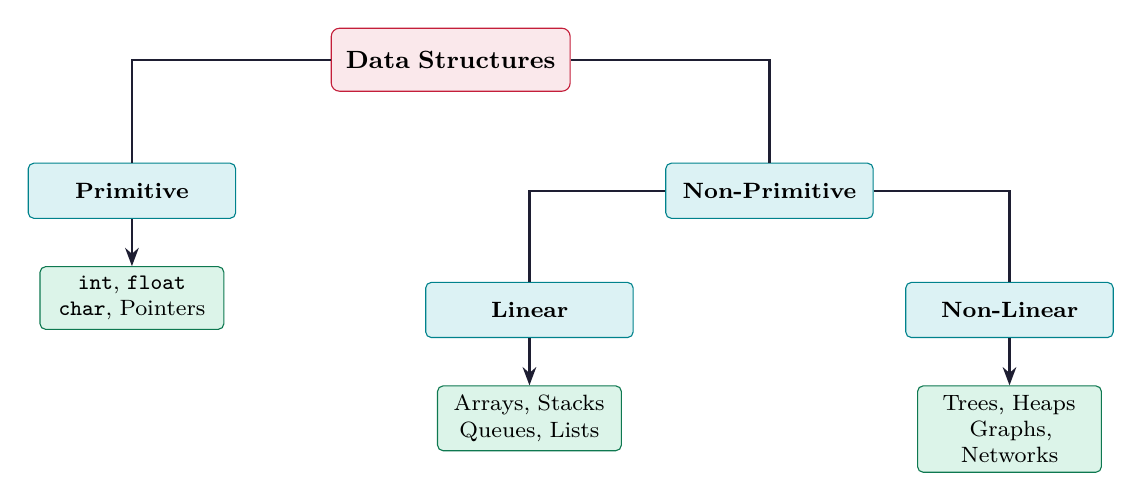
\begin{tikzpicture}[
  node distance=0.8cm and 0.6cm,
  every node/.style={font=\footnotesize},
  root/.style={rectangle, draw=myred, fill=hdrred, font=\small\bfseries, rounded corners=3pt, text width=2.8cm, align=center, minimum height=0.8cm},
  cat/.style={rectangle, draw=myteal, fill=hdrteal, font=\footnotesize\bfseries, rounded corners=2pt, text width=2.4cm, align=center, minimum height=0.7cm},
  leaf/.style={rectangle, draw=mygreen, fill=hdrgreen, rounded corners=2pt, text width=2.1cm, align=center, minimum height=0.65cm}
]
  \node[root] (ds) {Data Structures};
  \node[cat, below left=0.9cm and 1.2cm of ds] (prim) {Primitive};
  \node[cat, below right=0.9cm and 1.2cm of ds] (nonprim) {Non-Primitive};

  \draw[line] (ds) -| (prim);
  \draw[line] (ds) -| (nonprim);

  \node[leaf, below=0.6cm of prim] (p1) {\texttt{int}, \texttt{float}\\ \texttt{char}, Pointers};
  \draw[arrow] (prim) -- (p1);

  \node[cat, below left=0.8cm and 0.4cm of nonprim] (lin) {Linear};
  \node[cat, below right=0.8cm and 0.4cm of nonprim] (nonlin) {Non-Linear};

  \draw[line] (nonprim) -| (lin);
  \draw[line] (nonprim) -| (nonlin);

  \node[leaf, below=0.6cm of lin] (l1) {Arrays, Stacks\\ Queues, Lists};
  \node[leaf, below=0.6cm of nonlin] (nl1) {Trees, Heaps\\ Graphs, Networks};

  \draw[arrow] (lin) -- (l1);
  \draw[arrow] (nonlin) -- (nl1);
\end{tikzpicture}
\end{tcolorbox}

\subsection{Fundamental Data Structure Operations}
Every computational structure supports standard operational primitives:
\begin{enumerate}[leftmargin=*, itemsep=2pt]
  \item \textbf{Traversing:} Accessing each stored element exactly once to process or display data.
  \item \textbf{Insertion:} Adding a new data element at a designated index, boundary, or ordered position.
  \item \textbf{Deletion:} Removing an existing data item and releasing or compacting memory.
  \item \textbf{Searching:} Finding the memory address or index of an element satisfying a target search key.
  \item \textbf{Sorting:} Permuting elements into a monotonic ascending or descending collation order.
  \item \textbf{Merging:} Combining two distinct ordered datasets into a unified ordered sequence.
\end{enumerate}

\subsection{Array Memory Representations and Address Calculation}
An array is a homogeneous, contiguous collection of items accessed via integer offsets.
\par\vspace{4pt}\noindent
Let:
\begin{itemize}[leftmargin=*, nosep]
  \item $B = \text{Base Address}$ (memory address of the first byte of the array),
  \item $W = \text{Size of each element in bytes (word size)}$,
  \item $LB = \text{Lower Bound of indices}$ (default is $0$ in C, $1$ in mathematical texts).
\end{itemize}

\begin{tcolorbox}[formulabox, title={\textbf{Address Calculation Formulas for Multi-Dimensional Arrays}}]
\textbf{1. One-Dimensional Array $A[LB \dots UB]$:}
\begin{equation}
  \text{Loc}(A[i]) = B + W \cdot (i - LB)
\end{equation}

\textbf{2. Two-Dimensional Array $A[LB_1 \dots UB_1, \; LB_2 \dots UB_2]$:}\\
Let $N_1 = UB_1 - LB_1 + 1$ (total rows) and $N_2 = UB_2 - LB_2 + 1$ (total columns).
\begin{itemize}[leftmargin=*, itemsep=3pt]
  \item \textbf{Row-Major Order (RMO)} (consecutive row elements stored adjacently):
  \begin{equation}
    \text{Loc}(A[i][j]) = B + W \cdot \Big[ (i - LB_1) \cdot N_2 + (j - LB_2) \Big]
  \end{equation}
  \item \textbf{Column-Major Order (CMO)} (consecutive column elements stored adjacently):
  \begin{equation}
    \text{Loc}(A[i][j]) = B + W \cdot \Big[ (j - LB_2) \cdot N_1 + (i - LB_1) \Big]
  \end{equation}
\end{itemize}
\end{tcolorbox}

\begin{tcolorbox}[examplebox, title={\textbf{Exam Numerical: 2D Array Address Calculation}}]
\textbf{Problem:} An array $A[-5 \dots 15, \; 10 \dots 40]$ is allocated in byte-addressed RAM starting at base address $B = 1024$. Each element occupies $W = 4$ bytes. Determine the memory location of element $A[3][25]$ under both Row-Major and Column-Major storage schemes.
\par\vspace{4pt}
\textbf{Solution:}
\begin{itemize}[leftmargin=*, itemsep=2pt]
  \item $LB_1 = -5, \; UB_1 = 15 \implies N_1 = 15 - (-5) + 1 = 21$ rows.
  \item $LB_2 = 10, \; UB_2 = 40 \implies N_2 = 40 - 10 + 1 = 31$ columns.
  \item Row offset: $i - LB_1 = 3 - (-5) = 8$.
  \item Column offset: $j - LB_2 = 25 - 10 = 15$.
\end{itemize}
\textbf{1. Under Row-Major Order (RMO):}
\begin{align*}
  \text{Loc}(A[3][25]) &= 1024 + 4 \cdot [8 \cdot 31 + 15] = 1024 + 4 \cdot [248 + 15] \\
  &= 1024 + 4 \cdot 263 = 1024 + 1052 = \mathbf{2076}
\end{align*}
\textbf{2. Under Column-Major Order (CMO):}
\begin{align*}
  \text{Loc}(A[3][25]) &= 1024 + 4 \cdot [15 \cdot 21 + 8] = 1024 + 4 \cdot [315 + 8] \\
  &= 1024 + 4 \cdot 323 = 1024 + 1292 = \mathbf{2316}
\end{align*}
\end{tcolorbox}

% ───────────────────────────────────────────────────────────────────────────────
\section{Algorithm Analysis and Performance Metrics}
% ───────────────────────────────────────────────────────────────────────────────

\begin{tcolorbox}[defbox, title={\textbf{Definition: Algorithm Criteria and Formal Characteristics}}]
An \textbf{algorithm} is a finite, unambiguous, step-by-step computational procedure that accepts an initial input set and transforms it into a deterministic output set. Formally, every valid algorithm must satisfy:
\begin{enumerate}[leftmargin=*, nosep]
  \item \textbf{Input:} Generates output from zero or more well-defined external inputs.
  \item \textbf{Output:} Produces at least one quantifiable mathematical or logical result.
  \item \textbf{Definiteness:} Every operational step is completely clear, rigorous, and unambiguous.
  \item \textbf{Finiteness:} Terminates strictly after a finite number of executable instructions for all valid inputs.
  \item \textbf{Effectiveness:} Every instruction is basic enough to be executed exactly in finite time (feasible on physical hardware).
\end{enumerate}
\end{tcolorbox}

\subsection{Performance Metrics: Time and Space Complexity}
Algorithmic efficiency is measured independently of machine clock speed, compiler optimizations, or operating system jitter:
\begin{itemize}[leftmargin=*, itemsep=4pt]
  \item \textbf{Space Complexity $S(P)$:} Total memory consumed by program $P$ over its execution lifecycle:
  \begin{equation}
    S(P) = c + S_{\text{variable}}(I)
  \end{equation}
  where $c$ is the fixed part (instruction space, constants, scalar variables) and $S_{\text{variable}}(I)$ is the instance-dependent variable part (dynamically allocated memory, recursion stack activation frames).
  \item \textbf{Time Complexity $T(P)$:} Total computational operations or instruction steps executed as a mathematical function of input problem size $n$.
\end{itemize}

\subsection{Frequency Count Method}
The frequency count determines how many times each statement executes:
\begin{tcolorbox}[examplebox, title={\textbf{Step-Count Analysis of Nested Loops}}]
Consider the matrix multiplication algorithm for two $n \times n$ matrices:
\begin{verbatim}
for (i = 0; i < n; i++)                 // Executes n + 1 times
    for (j = 0; j < n; j++)             // Executes n * (n + 1) times
    {
        C[i][j] = 0;                    // Executes n * n times
        for (k = 0; k < n; k++)         // Executes n * n * (n + 1) times
            C[i][j] += A[i][k]*B[k][j]; // Executes n * n * n times
    }
\end{verbatim}
Total inner statement execution count: $f(n) = n^3$. As $n \to \infty$, the cubic term dominates all lower-order terms, yielding a time complexity of $\Theta(n^3)$.
\end{tcolorbox}

% ───────────────────────────────────────────────────────────────────────────────
\section{Asymptotic Notations and Growth of Functions}
% ───────────────────────────────────────────────────────────────────────────────

\begin{tcolorbox}[defbox, title={\textbf{Formal Definitions of Asymptotic Bounds}}]
Let $f(n)$ and $g(n)$ be asymptotically non-negative functions defined on the set of natural numbers $\mathbb{N}$.
\par\vspace{4pt}
\begin{enumerate}[leftmargin=*, itemsep=4pt]
  \item \textbf{Big-O Notation ($\mathcal{O}$ --- Asymptotic Upper Bound):}
  \begin{equation}
    \mathcal{O}(g(n)) = \big\{ f(n) : \exists\; c > 0, \; n_0 \in \mathbb{N} \text{ such that } 0 \le f(n) \le c \cdot g(n) \;\; \forall\; n \ge n_0 \big\}
  \end{equation}
  \item \textbf{Big-Omega Notation ($\Omega$ --- Asymptotic Lower Bound):}
  \begin{equation}
    \Omega(g(n)) = \big\{ f(n) : \exists\; c > 0, \; n_0 \in \mathbb{N} \text{ such that } 0 \le c \cdot g(n) \le f(n) \;\; \forall\; n \ge n_0 \big\}
  \end{equation}
  \item \textbf{Big-Theta Notation ($\Theta$ --- Asymptotically Tight Bound):}
  \begin{equation}
    \Theta(g(n)) = \big\{ f(n) : \exists\; c_1, c_2 > 0, \; n_0 \in \mathbb{N} \text{ s.t. } 0 \le c_1 g(n) \le f(n) \le c_2 g(n) \;\; \forall\; n \ge n_0 \big\}
  \end{equation}
\end{enumerate}
\end{tcolorbox}

\begin{tcolorbox}[tikzbox, title={\textbf{Geometric Interpretation of Asymptotic Notations}}]
\centering
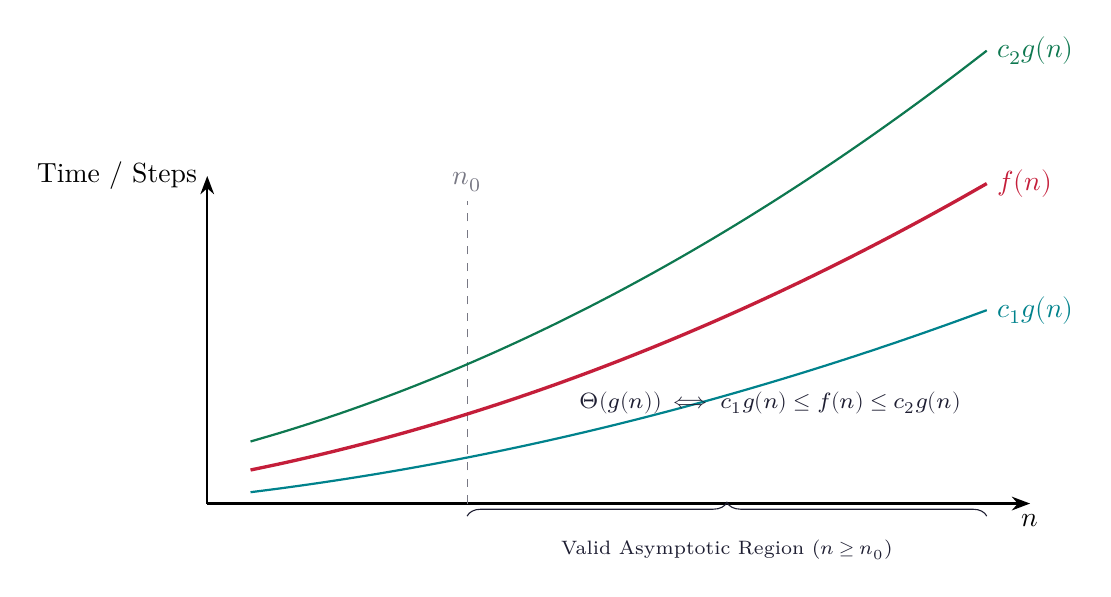
\begin{tikzpicture}[xscale=1.1, yscale=0.8]
  % Axes
  \draw[-Stealth, thick] (0,0) -- (9.5,0) node[below] {$n$};
  \draw[-Stealth, thick] (0,0) -- (0,5.2) node[left] {Time / Steps};

  % Threshold line n_0
  \draw[dashed, mydark!60] (3.0,0) -- (3.0,4.8) node[above] {$n_0$};

  % Big-Theta Curves
  \draw[domain=0.5:9, smooth, variable=\x, thick, color=mygreen] plot ({\x}, {0.35*\x + 0.04*\x*\x + 0.8}) node[right] {$c_2 g(n)$};
  \draw[domain=0.5:9, smooth, variable=\x, very thick, color=myred] plot ({\x}, {0.25*\x + 0.03*\x*\x + 0.4}) node[right] {$f(n)$};
  \draw[domain=0.5:9, smooth, variable=\x, thick, color=myteal] plot ({\x}, {0.15*\x + 0.02*\x*\x + 0.1}) node[right] {$c_1 g(n)$};

  % Shaded region
  \node[font=\footnotesize, color=mydark] at (6.5,1.6) {$\Theta(g(n)) \iff c_1 g(n) \le f(n) \le c_2 g(n)$};
  \draw[decorate, decoration={brace, amplitude=5pt}, mydark] (3.0,-0.2) -- (9.0,-0.2) node[midway, below=5pt, font=\scriptsize] {Valid Asymptotic Region ($n \ge n_0$)};
\end{tikzpicture}
\end{tcolorbox}

\subsection{Little-o and Little-omega Notations}
\begin{itemize}[leftmargin=*, itemsep=3pt]
  \item \textbf{Little-o Notation ($o$ --- Strict Upper Bound):}
  \begin{equation}
    f(n) = o(g(n)) \iff \lim_{n \to \infty} \frac{f(n)}{g(n)} = 0
  \end{equation}
  Unlike $\mathcal{O}$, $f(n)$ cannot be asymptotically equal to $g(n)$ (e.g., $2n = o(n^2)$, but $2n \ne o(n)$).
  \item \textbf{Little-omega Notation ($\omega$ --- Strict Lower Bound):}
  \begin{equation}
    f(n) = \omega(g(n)) \iff \lim_{n \to \infty} \frac{f(n)}{g(n)} = \infty
  \end{equation}
\end{itemize}

\subsection{Hierarchy and Properties of Growth Rates}
Standard asymptotic complexities scale monotonically:
\begin{align}
  \mathcal{O}(1) &< \mathcal{O}(\log \log n) < \mathcal{O}(\log n) < \mathcal{O}(\sqrt{n}) < \mathcal{O}(n) \notag\\
  &< \mathcal{O}(n \log n) < \mathcal{O}(n^2) < \mathcal{O}(n^3) < \mathcal{O}(2^n) < \mathcal{O}(n!) < \mathcal{O}(n^n)
\end{align}

\par\vspace{4pt}\noindent
\textbf{Fundamental Algebraic Properties:}
\begin{itemize}[leftmargin=*, itemsep=2pt]
  \item \textbf{Transitivity:} If $f(n) = \Theta(g(n))$ and $g(n) = \Theta(h(n))$, then $f(n) = \Theta(h(n))$.
  \item \textbf{Symmetry:} $f(n) = \Theta(g(n)) \iff g(n) = \Theta(f(n))$.
  \item \textbf{Transpose Symmetry:} $f(n) = \mathcal{O}(g(n)) \iff g(n) = \Omega(f(n))$.
  \item \textbf{Theorem:} $f(n) = \Theta(g(n)) \iff f(n) = \mathcal{O}(g(n)) \text{ and } f(n) = \Omega(g(n))$.
\end{itemize}

\subsection{The Time-Space Trade-Off}
In computational engineering, the \textbf{Time-Space Trade-off} dictates that algorithmic runtime can often be reduced at the expense of higher auxiliary memory usage, and vice-versa.
\begin{itemize}[leftmargin=*, itemsep=3pt]
  \item \textbf{Memory-Heavy, Fast Execution:} Hash tables provide $\mathcal{O}(1)$ average lookup by utilizing extra array buckets. Pre-computed lookup tables or memoization arrays in Dynamic Programming trade space to eliminate redundant exponential recursive calls.
  \item \textbf{Memory-Light, Slow Execution:} In-place algorithms with $\mathcal{O}(1)$ auxiliary space (e.g., linear scanning or recomputing values on demand) save RAM at the cost of $\mathcal{O}(n)$ or $\mathcal{O}(n^2)$ processing delays.
\end{itemize}

% ───────────────────────────────────────────────────────────────────────────────
\section{Searching Techniques and Algorithmic Complexity}
% ───────────────────────────────────────────────────────────────────────────────

\subsection{Linear (Sequential) Search}
Linear search scans an unsorted array sequentially from index $0$ to $n-1$, checking each element against target key $K$.

\begin{tcolorbox}[formulabox, title={\textbf{Linear Search Algorithm and Complexity Proof}}]
\textbf{Algorithm LinearSearch($A, n, K$):}
\begin{enumerate}[leftmargin=*, nosep]
  \item For $i = 0$ to $n - 1$ do:
  \item \quad If $A[i] == K$, return index $i$.
  \item Return $-1$ (Search Key Not Found).
\end{enumerate}
\par\vspace{4pt}\noindent
\textbf{Complexity Derivation:}
\begin{itemize}[leftmargin=*, itemsep=2pt]
  \item \textbf{Best-Case Time Complexity:} Target key is at the first index ($A[0] == K$). Requires $1$ comparison:
  \begin{equation}
    T_{\text{best}}(n) = \mathcal{O}(1)
  \end{equation}
  \item \textbf{Worst-Case Time Complexity:} Target key is at the last index ($A[n-1]$) or absent from array. Requires $n$ comparisons:
  \begin{equation}
    T_{\text{worst}}(n) = \mathcal{O}(n)
  \end{equation}
  \item \textbf{Average-Case Time Complexity:} Assuming uniform distribution where key is present with probability $p$, and equally likely at any position ($1/n$):
  \begin{equation}
    T_{\text{avg}}(n) = \sum_{i=1}^n i \cdot P(\text{found at } i) = \sum_{i=1}^n i \cdot \frac{1}{n} = \frac{1}{n} \cdot \frac{n(n+1)}{2} = \frac{n+1}{2} \implies \mathcal{O}(n)
  \end{equation}
  \item \textbf{Auxiliary Space:} $\mathcal{O}(1)$ (in-place search).
\end{itemize}
\end{tcolorbox}

\subsection{Binary Search Technique}
Binary search operates on a \textbf{monotonically sorted} contiguous sequence via divide-and-conquer, halving the search space in each iteration.

\begin{tcolorbox}[defbox, title={\textbf{Binary Search Algorithm (Iterative Implementation)}}]
\textbf{Algorithm BinarySearch($A, n, K$):}
\begin{enumerate}[leftmargin=*, nosep]
  \item Set $\text{low} = 0, \; \text{high} = n - 1$.
  \item While $\text{low} \le \text{high}$ do:
  \item \quad Compute $\text{mid} = \text{low} + \lfloor (\text{high} - \text{low})/2 \rfloor$. \quad \textit{(Prevents integer overflow)}
  \item \quad If $A[\text{mid}] == K$, return $\text{mid}$ (Success).
  \item \quad Else if $A[\text{mid}] < K$, set $\text{low} = \text{mid} + 1$.
  \item \quad Else set $\text{high} = \text{mid} - 1$.
  \item Return $-1$ (Key Absent).
\end{enumerate}
\end{tcolorbox}

\begin{tcolorbox}[tikzbox, title={\textbf{Decision Tree Representation of Binary Search on $n=7$ Elements}}]
\centering
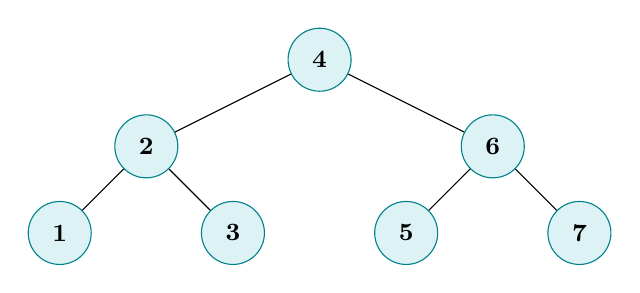
\begin{tikzpicture}[
  level distance=1.1cm,
  level 1/.style={sibling distance=4.4cm},
  level 2/.style={sibling distance=2.2cm},
  every node/.style={circle, draw=myteal, fill=hdrteal, font=\small\bfseries, inner sep=2pt, minimum size=0.8cm}
]
  \node {4}
    child { node {2}
      child { node {1} }
      child { node {3} }
    }
    child { node {6}
      child { node {5} }
      child { node {7} }
    };
\end{tikzpicture}
\par\vspace{2pt}
{\footnotesize At each stage, one comparison reduces the remaining search tree depth by 1. Total depth is $\lfloor \log_2 n \rfloor + 1$.}
\end{tcolorbox}

\begin{tcolorbox}[formulabox, title={\textbf{Binary Search Recurrence Relation and Complexity Derivation}}]
In each step, the algorithm performs $\mathcal{O}(1)$ comparisons and reduces problem size $n$ to $n/2$:
\begin{equation}
  T(n) = T\left(\frac{n}{2}\right) + c, \qquad T(1) = 1
\end{equation}
\textbf{Solving via Repeated Substitution (Unfolding):}
\begin{align*}
  T(n) &= T\left(\frac{n}{2}\right) + c = \left[T\left(\frac{n}{4}\right) + c\right] + c = T\left(\frac{n}{2^2}\right) + 2c \\
       &= T\left(\frac{n}{2^k}\right) + k \cdot c
\end{align*}
The process terminates when the subproblem reaches size 1: $\frac{n}{2^k} = 1 \implies 2^k = n \implies k = \log_2 n$.
\begin{equation}
  T(n) = T(1) + c \cdot \log_2 n = 1 + c \log_2 n \implies \mathbf{\Theta(\log_2 n)}
\end{equation}
\par\vspace{2pt}\noindent
\textbf{Summary of Bounds:}
\begin{itemize}[leftmargin=*, nosep]
  \item \textbf{Best-Case:} $A[\text{mid}] == K$ on first comparison $\implies \mathbf{\mathcal{O}(1)}$.
  \item \textbf{Worst-Case:} Element is at the leaf of the decision tree or absent $\implies \mathbf{\mathcal{O}(\log_2 n)}$.
  \item \textbf{Average-Case:} Successful search across all decision tree nodes $\implies \mathbf{\mathcal{O}(\log_2 n)}$.
  \item \textbf{Space Complexity:} $\mathcal{O}(1)$ for iterative version; $\mathcal{O}(\log_2 n)$ stack frames for recursive version.
\end{itemize}
\end{tcolorbox}

\subsection{Comparison: Linear Search vs Binary Search}
\par\vspace{6pt}\noindent
\begingroup
\setlength{\tabcolsep}{4.5pt}
\setlength{\extrarowheight}{3pt}
\renewcommand{\arraystretch}{1.35}
\begin{tabularx}{\linewidth}{|B{3.2cm}|Y|Y|}
\hline
\textbf{Criterion} & \textbf{Linear Search} & \textbf{Binary Search} \\
\hline
Prerequisite & Elements can be arbitrary/unsorted & Sequence \textbf{must} be monotonically sorted \\
\hline
Access Requirement & Sequential or Random access (Array or Linked List) & Random access required (Arrays only; inefficient on linked lists) \\
\hline
Best-Case Time & $\mathcal{O}(1)$ (first item matches) & $\mathcal{O}(1)$ (middle item matches) \\
\hline
Worst-Case Time & $\mathcal{O}(n)$ & $\mathcal{O}(\log_2 n)$ \\
\hline
Average-Case Time & $\mathcal{O}(n)$ & $\mathcal{O}(\log_2 n)$ \\
\hline
Space Complexity & $\mathcal{O}(1)$ in-place & $\mathcal{O}(1)$ iterative, $\mathcal{O}(\log n)$ recursive \\
\hline
Hardware Efficiency & Excellent CPU cache spatial locality & Multiple cache misses on large data jumps \\
\hline
Algorithm Paradigm & Brute-force linear scan & Divide-and-Conquer \\
\hline
\end{tabularx}
\endgroup

\newpage
% ===============================================================================
% MANDATORY QUICK REVISION PAGE
% ===============================================================================
\begin{center}
  {\large\bfseries\color{myred} Quick Revision --- Module 1}\\[3pt]
  {\small\color{mydark} Introduction, Algorithm Analysis and Searching Techniques $|$ ES-CS301}
\end{center}
\noindent{\color{myred}\rule{\linewidth}{1.2pt}}
\vspace{4pt}

\begin{tcolorbox}[formulabox, title={\textbf{Key Formulas and Asymptotic Relations at a Glance}}]
\renewcommand{\arraystretch}{1.25}
\begin{tabularx}{\linewidth}{B{5.0cm} X}
1D Array Address & $\text{Loc}(A[i]) = B + W \cdot (i - LB)$ \\[2pt]
2D Row-Major Address & $\text{Loc}(A[i][j]) = B + W \cdot [(i - LB_1) \cdot N_2 + (j - LB_2)]$ \\[2pt]
2D Column-Major Address & $\text{Loc}(A[i][j]) = B + W \cdot [(j - LB_2) \cdot N_1 + (i - LB_1)]$ \\[2pt]
Asymptotic Bounds ($\mathcal{O}, \Omega, \Theta$) & $f(n) \le c_1 g(n) \;(\mathcal{O}), \quad c_2 g(n) \le f(n) \;(\Omega), \quad c_3 g(n) \le f(n) \le c_4 g(n) \;(\Theta)$ \\[2pt]
Strict Limits ($o, \omega$) & $\lim_{n \to \infty} \frac{f(n)}{g(n)} = 0 \;(o), \quad \lim_{n \to \infty} \frac{f(n)}{g(n)} = \infty \;(\omega)$ \\[2pt]
Binary Search Recurrence & $T(n) = T(n/2) + \Theta(1) \implies T(n) = \Theta(\log_2 n)$ \\[2pt]
Linear Search Bounds & $\text{Best-Case: } \mathcal{O}(1), \quad \text{Worst-Case / Average: } \mathcal{O}(n)$ \\[2pt]
Complexity Hierarchy & $\mathcal{O}(1) < \mathcal{O}(\log n) < \mathcal{O}(n) < \mathcal{O}(n \log n) < \mathcal{O}(n^2) < \mathcal{O}(2^n) < \mathcal{O}(n!)$ \\[2pt]
\end{tabularx}
\end{tcolorbox}

\begin{tcolorbox}[defbox, title={\textbf{One-Line Definitions}}]
\begin{itemize}[leftmargin=*, itemsep=2pt, topsep=0pt]
  \item \textbf{Data Structure:} A logical and mathematical organization of data elements along with designated legal operations.
  \item \textbf{Abstract Data Type (ADT):} A mathematical model for data types defining behavior from user perspective without implementation details.
  \item \textbf{Linear Data Structure:} A data structure where elements form an ordered sequential sequence with 1-to-1 adjacent relations.
  \item \textbf{Row-Major Order (RMO):} A 2D mapping layout where all elements of row $i$ precede row $i+1$ in contiguous physical memory.
  \item \textbf{Column-Major Order (CMO):} A 2D mapping layout where all elements of column $j$ precede column $j+1$ in contiguous physical memory.
  \item \textbf{Big-O ($\mathcal{O}$):} An asymptotic notation defining a formal mathematical upper bound on algorithm computational growth.
  \item \textbf{Time-Space Trade-off:} The engineering principle where computational runtime is decreased by allocating extra memory.
  \item \textbf{Binary Search:} A divide-and-conquer algorithm on sorted arrays halving search space in $\mathcal{O}(\log_2 n)$ comparisons.
\end{itemize}
\end{tcolorbox}

\newpage

\begin{tcolorbox}[exambox, title={\textbf{Frequently Asked / Viva Questions (Part 1)}}]
\begin{enumerate}[topsep=0pt, label=\textbf{Q\arabic*.}, itemsep=4pt]
  \item \Q{What is the difference between a Data Type and a Data Structure?}
  A data type is a primitive classification defining a set of values and allowable low-level hardware operations (e.g., \texttt{int}, \texttt{float}). A data structure is a higher-level collection of data elements organized logically with specific algorithms to store and manipulate them efficiently in memory (e.g., arrays, stacks, trees).

  \item \Q{Why do we prefer asymptotic notations over clock time for analyzing algorithms?}
  Physical clock time depends on machine architecture, processor speed, compiler optimizations, background processes, and cache memory. Asymptotic notations evaluate performance purely as a function of input size $n$, independent of hardware, providing an objective, universal measure of scalability.

  \item \Q{State the necessary and sufficient condition for $f(n) = \Theta(g(n))$.}
  The function $f(n) = \Theta(g(n))$ if and only if $f(n) = \mathcal{O}(g(n))$ and $f(n) = \Omega(g(n))$. That is, $g(n)$ serves simultaneously as both the asymptotic upper bound and lower bound within positive constant multipliers $c_1$ and $c_2$.

  \item \Q{Why must an array be sorted prior to executing Binary Search?}
  Binary search relies on the monotonicity of elements. When the target key $K$ is compared with the middle element $A[\text{mid}]$, the algorithm assumes that all elements to the left are $\le A[\text{mid}]$ and all elements to the right are $\ge A[\text{mid}]$. Without sorted order, discarding half the array could eliminate the target key.

  \item \Q{Why is Binary Search inefficient when applied to a Singly Linked List?}
  Binary search requires finding the midpoint in $\mathcal{O}(1)$ time. In a linked list, random access is not supported ($A[i]$ takes $\mathcal{O}(i)$ traversal steps). Locating the middle node takes $\mathcal{O}(n)$ time, which negates the divide-and-conquer speedup, resulting in overall $\mathcal{O}(n)$ complexity.

  \item \Q{Explain the concept of integer overflow in computing the midpoint in Binary Search and how it is resolved.}
  Writing \texttt{mid = (low + high) / 2} can cause integer overflow if the sum \texttt{low + high} exceeds the maximum 32-bit signed integer value ($2^{31}-1$). The overflow wraps to a negative number, causing an index out-of-bounds fault. It is avoided using \texttt{mid = low + (high - low) / 2}.

  \item \Q{Differentiate between Big-O ($\mathcal{O}$) and Little-o ($o$).}
  Big-O establishes an asymptotic upper bound that may be tight ($2n^2 = \mathcal{O}(n^2)$ is valid). Little-o establishes a strict, non-tight upper bound such that $f(n)$ grows strictly slower than $g(n)$ as $n \to \infty$ ($\lim_{n \to \infty} f(n)/g(n) = 0$). Thus $2n = o(n^2)$, but $2n^2 \ne o(n^2)$.
\end{enumerate}
\end{tcolorbox}

\newpage

\begin{tcolorbox}[exambox, title={\textbf{Frequently Asked / Viva Questions (Part 2)}}]
\begin{enumerate}[topsep=0pt, label=\textbf{Q\arabic*.}, itemsep=4pt, start=8]
  \item \Q{What is the difference between Space Complexity and Auxiliary Space?}
  Space complexity is the total memory used by an algorithm, including both the input data and any extra working memory. Auxiliary space refers exclusively to the extra temporary or scratchpad memory allocated by the algorithm beyond the input size.

  \item \Q{Provide an example of an engineering Time-Space trade-off.}
  In calculating Fibonacci numbers: naive recursion takes $\mathcal{O}(2^n)$ time and $\mathcal{O}(n)$ call-stack space. Using dynamic programming memoization with an auxiliary array of size $n$, runtime drops dramatically to $\mathcal{O}(n)$ time at the expense of $\mathcal{O}(n)$ extra storage space.

  \item \Q{What are the worst-case, best-case, and average-case scenarios for Linear Search?}
  Best case is $\mathcal{O}(1)$ (element found at index $0$). Worst case is $\mathcal{O}(n)$ (element is at index $n-1$ or absent). Average case is $\mathcal{O}(n)$ (specifically $(n+1)/2$ comparisons under a uniform random distribution).
\end{enumerate}
\end{tcolorbox}

\vspace{3pt}

\begin{tcolorbox}[tikzbox, title={\textbf{Summary Matrix: Comprehensive Comparison of Searching and Analysis Fundamentals}}]
\par\vspace{2pt}\noindent
\begingroup
\footnotesize
\setlength{\tabcolsep}{3.5pt}
\setlength{\extrarowheight}{1.5pt}
\renewcommand{\arraystretch}{1.15}
\begin{tabularx}{\linewidth}{|B{2.4cm}|B{3.2cm}|B{2.8cm}|Y|}
\hline
\textbf{Topic / Technique} & \textbf{Core Governing Relation} & \textbf{Complexity Bound} & \textbf{Key Engineering Takeaway} \\
\hline
Row-Major 2D Addressing & $\text{Loc} = B + W[(i-LB_1)N_2 + (j-LB_2)]$ & $\mathcal{O}(1)$ compute time & C/C++ memory layout; row iteration preserves cache locality. \\
\hline
Column-Major 2D Addressing & $\text{Loc} = B + W[(j-LB_2)N_1 + (i-LB_1)]$ & $\mathcal{O}(1)$ compute time & Fortran/MATLAB layout; column-by-column iteration preferred. \\
\hline
Big-O Notation ($\mathcal{O}$) & $f(n) \le c \cdot g(n) \;\; \forall n \ge n_0$ & Upper bound & Worst-case computational ceiling guarantees. \\
\hline
Big-Theta Notation ($\Theta$) & $c_1 g(n) \le f(n) \le c_2 g(n)$ & Tight bound & Exact algorithmic rate of growth. \\
\hline
Linear Search & Sequential traversal $A[0 \dots n-1]$ & Worst: $\mathcal{O}(n)$, Best: $\mathcal{O}(1)$ & Unsorted or small lists; works natively on linked lists. \\
\hline
Binary Search & $T(n) = T(n/2) + \mathcal{O}(1)$ & Worst: $\mathcal{O}(\log n)$, Best: $\mathcal{O}(1)$ & Strictly requires sorted array and random access memory. \\
\hline
\end{tabularx}
\endgroup
\end{tcolorbox}


% -- Module 2 -----------------------------------------------------------------
\modulestart{2}{Abstract Data Type Stack and Fundamental Operations}

\section{Abstract Data Type Stack and Fundamental Operations}
% ───────────────────────────────────────────────────────────────────────────────

\begin{tcolorbox}[defbox, title={\textbf{Definition: Stack Abstract Data Type (ADT)}}]
A \textbf{Stack} is a linear, restricted-access data structure adhering strictly to the \textbf{Last-In, First-Out (LIFO)} or \textbf{First-In, Last-Out (FILO)} operating discipline. All insertions (\texttt{push}) and deletions (\texttt{pop}) are constrained to take place at a single end termed the \textbf{Top of Stack (TOS)}.
\par\vspace{4pt}
Formally, a Stack $S$ over an element domain $E$ is defined by:
\begin{itemize}[leftmargin=*, nosep]
  \item State: An ordered sequence $S = \langle e_0, e_1, \dots, e_k \rangle$ where $e_k$ is the Top element.
  \item Auxiliary Pointer: An integer index $\text{top} \in [-1, \text{MAX}-1]$ indicating the index of the most recently inserted item.
\end{itemize}
\end{tcolorbox}

\subsection{Array Implementation of Stack}
In an array-based static implementation, elements reside in contiguous storage $S[0 \dots \text{MAX}-1]$.
\begin{itemize}[leftmargin=*, itemsep=3pt]
  \item \textbf{Initial Condition:} $\text{top} = -1$ (stack is strictly empty).
  \item \textbf{Stack Overflow Condition:} Attempting to insert an element when the physical capacity is exhausted:
  \begin{equation}
    \text{Overflow} \iff \text{top} == \text{MAX} - 1
  \end{equation}
  \item \textbf{Stack Underflow Condition:} Attempting to retrieve or delete an element from an empty stack:
  \begin{equation}
    \text{Underflow} \iff \text{top} == -1
  \end{equation}
\end{itemize}

\begin{tcolorbox}[formulabox, title={\textbf{Core Stack Primitive Algorithms and Complexity Bounds}}]
\textbf{1. Algorithm Push($S, \text{top}, x$):}
\begin{verbatim}
if (top == MAX - 1)
    report "Stack Overflow" and exit error;
top = top + 1;
S[top] = x;
\end{verbatim}
Time Complexity: $\mathbf{\mathcal{O}(1)}$ \quad Space Complexity: $\mathbf{\mathcal{O}(1)}$

\par\vspace{3pt}\noindent
\textbf{2. Algorithm Pop($S, \text{top}$):}
\begin{verbatim}
if (top == -1)
    report "Stack Underflow" and exit error;
item = S[top];
top = top - 1;
return item;
\end{verbatim}
Time Complexity: $\mathbf{\mathcal{O}(1)}$ \quad Space Complexity: $\mathbf{\mathcal{O}(1)}$

\par\vspace{3pt}\noindent
\textbf{3. Algorithm Peek($S, \text{top}$):}
\begin{verbatim}
if (top == -1)
    report "Stack Empty" and exit error;
return S[top]; // Non-destructive inspection
\end{verbatim}
Time Complexity: $\mathbf{\mathcal{O}(1)}$ \quad Space Complexity: $\mathbf{\mathcal{O}(1)}$
\end{tcolorbox}

\begin{tcolorbox}[tikzbox, title={\textbf{LIFO Mechanism and State Transitions in Stack Operations}}]
\centering
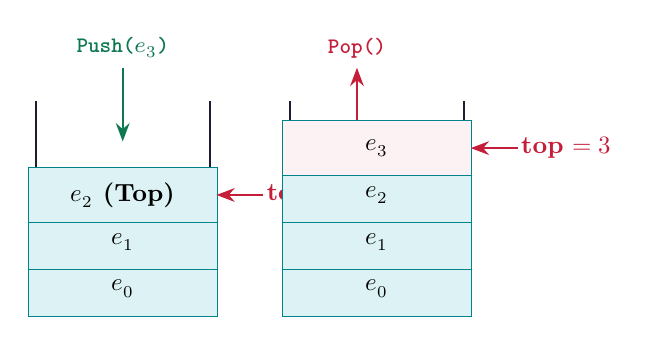
\begin{tikzpicture}[scale=0.85, every node/.style={font=\small}]
  % Stack slots
  \draw[thick, mydark] (0,3.2) -- (0,0) -- (2.6,0) -- (2.6,3.2);
  \node[stackslot] at (1.3,0.4) {$e_0$};
  \node[stackslot] at (1.3,1.1) {$e_1$};
  \node[stackslot] at (1.3,1.8) {$e_2$ (Top)};

  \draw[redarrow] (3.4,1.8) -- (2.7,1.8) node[midway, right=6pt] {\textbf{top} $= 2$};

  % Push Action
  \draw[arrow, mygreen] (1.3,3.7) -- (1.3,2.6);
  \node[above, font=\footnotesize\bfseries, color=mygreen] at (1.3,3.7) {\texttt{Push($e_3$)}};

  % Pop Action
  \draw[arrow, myred] (4.8,2.6) -- (4.8,3.7);
  \node[above, font=\footnotesize\bfseries, color=myred] at (4.8,3.7) {\texttt{Pop()}};
  \draw[thick, mydark] (3.8,3.2) -- (3.8,0) -- (6.4,0) -- (6.4,3.2);
  \node[stackslot] at (5.1,0.4) {$e_0$};
  \node[stackslot] at (5.1,1.1) {$e_1$};
  \node[stackslot] at (5.1,1.8) {$e_2$};
  \node[stackslot, fill=hdrred!60] at (5.1,2.5) {$e_3$};
  \draw[redarrow] (7.2,2.5) -- (6.5,2.5) node[midway, right=6pt] {\textbf{top} $= 3$};
\end{tikzpicture}
\end{tcolorbox}

% ───────────────────────────────────────────────────────────────────────────────
\section{Applications of Stacks}
% ───────────────────────────────────────────────────────────────────────────────

\subsection{Arithmetic Expression Formats and Operator Precedence}
Mathematical expressions are represented in three distinct syntactic notations:
\begin{enumerate}[leftmargin=*, itemsep=3pt]
  \item \textbf{Infix Notation:} Binary operators are placed between operands: $\langle \text{Operand} \rangle \; \mathbf{Op} \; \langle \text{Operand} \rangle$ (e.g., $(A + B) * C$). Requires explicit parentheses and precedence parsing rules.
  \item \textbf{Postfix Notation (Reverse Polish Notation --- RPN):} Operators appear immediately following their operands: $\langle \text{Operand} \rangle \; \langle \text{Operand} \rangle \; \mathbf{Op}$ (e.g., $A B + C *$). Evaluated linearly without parentheses or backtrack searching.
  \item \textbf{Prefix Notation (Polish Notation):} Operators precede operands: $\mathbf{Op} \; \langle \text{Operand} \rangle \; \langle \text{Operand} \rangle$ (e.g., $* + A B C$).
\end{enumerate}

\par\vspace{6pt}\noindent
\begingroup
\setlength{\tabcolsep}{5pt}
\setlength{\extrarowheight}{3pt}
\renewcommand{\arraystretch}{1.3}
\begin{tabularx}{\linewidth}{|B{3.2cm}|B{3.5cm}|B{2.8cm}|Y|}
\hline
\textbf{Operator} & \textbf{Operation Description} & \textbf{Associativity} & \textbf{Precedence Rank} \\
\hline
\texttt{\^{}} or \texttt{\$} & Exponentiation & Right-to-Left ($\text{R} \to \text{L}$) & Highest (Rank 3) \\
\hline
\texttt{*}, \texttt{/}, \texttt{\%} & Multiplication, Division, Modulo & Left-to-Right ($\text{L} \to \text{R}$) & Intermediate (Rank 2) \\
\hline
\texttt{+}, \texttt{-} & Addition, Subtraction & Left-to-Right ($\text{L} \to \text{R}$) & Lowest (Rank 1) \\
\hline
\texttt{(} & Left Parenthesis & Left-to-Right & Rank 0 (Inside Stack) \\
\hline
\end{tabularx}
\endgroup

\subsection{Infix to Postfix Conversion Algorithm}
\begin{tcolorbox}[defbox, title={\textbf{Shunting-Yard Infix to Postfix Algorithm}}]
\begin{enumerate}[leftmargin=*, nosep]
  \item Initialize an empty operator stack $S$ and an empty postfix output string $P$.
  \item Scan the infix expression string $I$ from left to right, character by character:
  \begin{itemize}[leftmargin=*, nosep]
    \item \textbf{If Operand:} Append directly to postfix string $P$.
    \item \textbf{If Left Parenthesis \texttt{'('}:} Push onto stack $S$.
    \item \textbf{If Right Parenthesis \texttt{')'}:} Pop from $S$ and append to $P$ repeatedly until \texttt{'('} is popped. Discard both parentheses.
    \item \textbf{If Operator $op$:} While stack is non-empty, and $\text{Prec}(\text{top}) > \text{Prec}(op)$ (or $\text{Prec}(\text{top}) == \text{Prec}(op)$ with Left-Associativity), pop $S$ and append to $P$. Then push $op$ onto $S$.
  \end{itemize}
  \item After end of input string, pop all remaining operators from $S$ and append to $P$.
\end{enumerate}
\end{tcolorbox}

\begin{tcolorbox}[examplebox, title={\textbf{Step-by-Step Trace: Infix to Postfix Conversion}}]
Convert: $I = A + B * (C \wedge D - E) \wedge (F + G * H) - I$
\par\vspace{4pt}
\begingroup
\setlength{\tabcolsep}{4.5pt}
\setlength{\extrarowheight}{1.5pt}
\renewcommand{\arraystretch}{1.15}
\begin{tabularx}{\linewidth}{|B{1.6cm}|B{2.8cm}|Y|B{3.2cm}|}
\hline
\textbf{Token} & \textbf{Operator Stack} & \textbf{Postfix Output $P$} & \textbf{Action} \\
\hline
$A$ & $\emptyset$ & $A$ & Append operand \\
$+$ & $+$ & $A$ & Push operator \\
$B$ & $+$ & $A B$ & Append operand \\
$*$ & $+ \; *$ & $A B$ & Push (higher precedence) \\
$($ & $+ \; * \; ($ & $A B$ & Push parenthesis \\
$C$ & $+ \; * \; ($ & $A B C$ & Append operand \\
$\wedge$ & $+ \; * \; ( \; \wedge$ & $A B C$ & Push exponent \\
$D$ & $+ \; * \; ( \; \wedge$ & $A B C D$ & Append operand \\
$-$ & $+ \; * \; ( \; -$ & $A B C D \wedge$ & Pop $\wedge$, push $-$ \\
$E$ & $+ \; * \; ( \; -$ & $A B C D \wedge E$ & Append operand \\
$)$ & $+ \; *$ & $A B C D \wedge E -$ & Pop until $($, discard \\
$\wedge$ & $+ \; * \; \wedge$ & $A B C D \wedge E -$ & Push (higher precedence) \\
$($ & $+ \; * \; \wedge \; ($ & $A B C D \wedge E -$ & Push parenthesis \\
$F$ & $+ \; * \; \wedge \; ($ & $A B C D \wedge E - F$ & Append operand \\
$+$ & $+ \; * \; \wedge \; ( \; +$ & $A B C D \wedge E - F$ & Push operator \\
$G$ & $+ \; * \; \wedge \; ( \; +$ & $A B C D \wedge E - F G$ & Append operand \\
$*$ & $+ \; * \; \wedge \; ( \; + \; *$ & $A B C D \wedge E - F G$ & Push (higher precedence) \\
$H$ & $+ \; * \; \wedge \; ( \; + \; *$ & $A B C D \wedge E - F G H$ & Append operand \\
$)$ & $+ \; * \; \wedge$ & $A B C D \wedge E - F G H * +$ & Pop until $($, discard \\
$-$ & $-$ & $A B C D \wedge E - F G H * + \wedge * +$ & Pop $\wedge, *, +$, push $-$ \\
$I$ & $-$ & $A B C D \wedge E - F G H * + \wedge * + I$ & Append operand \\
\textbf{End} & $\emptyset$ & $\mathbf{A B C D \wedge E - F G H * + \wedge * + I -}$ & Pop all remaining \\
\hline
\end{tabularx}
\endgroup
\end{tcolorbox}

\subsection{Evaluation of Postfix Expressions}
\begin{tcolorbox}[formulabox, title={\textbf{Postfix Expression Evaluation Algorithm}}]
Scan postfix string $P$ from left to right:
\begin{enumerate}[leftmargin=*, nosep]
  \item If current symbol is an operand, push its numerical value onto operand stack $S$.
  \item If symbol is an operator $\odot$:
  \begin{itemize}[leftmargin=*, nosep]
    \item $\text{op}_2 = \text{Pop}(S)$ \quad \textit{(Second operand popped first!)}
    \item $\text{op}_1 = \text{Pop}(S)$ \quad \textit{(First operand popped second!)}
    \item Compute $\text{result} = \text{op}_1 \odot \text{op}_2$.
    \item $\text{Push}(S, \text{result})$.
  \end{itemize}
  \item When string ends, the final evaluated result resides at $\text{Pop}(S)$.
\end{enumerate}
Time Complexity: $\mathbf{\mathcal{O}(n)}$ \quad Auxiliary Space: $\mathbf{\mathcal{O}(n)}$
\end{tcolorbox}

\begin{tcolorbox}[examplebox, title={\textbf{Evaluation Trace: Numerical Postfix String}}]
Evaluate: $P = 6 \; 2 \; 3 \; + \; * \; 12 \; 4 \; / \; -$
\begin{itemize}[leftmargin=*, itemsep=2pt]
  \item Scan \texttt{6}, \texttt{2}, \texttt{3}: Push to stack $\implies S = [6, 2, 3]$.
  \item Encounter \texttt{+}: Pop $\text{op}_2 = 3$, $\text{op}_1 = 2$. Compute $2 + 3 = 5$. Push $5 \implies S = [6, 5]$.
  \item Encounter \texttt{*}: Pop $\text{op}_2 = 5$, $\text{op}_1 = 6$. Compute $6 * 5 = 30$. Push $30 \implies S = [30]$.
  \item Scan \texttt{12}, \texttt{4}: Push to stack $\implies S = [30, 12, 4]$.
  \item Encounter \texttt{/}: Pop $\text{op}_2 = 4$, $\text{op}_1 = 12$. Compute $12 / 4 = 3$. Push $3 \implies S = [30, 3]$.
  \item Encounter \texttt{-}: Pop $\text{op}_2 = 3$, $\text{op}_1 = 30$. Compute $30 - 3 = 27$. Push $27 \implies S = [27]$.
  \item End of expression: Final Result = $\mathbf{27}$.
\end{itemize}
\end{tcolorbox}

\subsection{Infix to Prefix Conversion and Prefix Evaluation}
\begin{tcolorbox}[defbox, title={\textbf{Infix to Prefix Conversion Algorithm (Reversal Method)}}]
To convert an infix expression $I$ to prefix notation $Pre$:
\begin{enumerate}[leftmargin=*, nosep]
  \item Reverse the infix string $I$.
  \item In the reversed string, replace every \texttt{'('} with \texttt{')'} and every \texttt{')'} with \texttt{'('}.
  \item Compute the postfix expression of this transformed string using the Shunting-Yard algorithm (with operator precedence rules: if precedence of scanned operator equals TOS, operators with right-associativity pop TOS, left-associative operators are pushed).
  \item Reverse the resulting postfix string. The final string is the valid \textbf{Prefix expression}.
\end{enumerate}
Time Complexity: $\mathbf{\mathcal{O}(n)}$ \quad Auxiliary Space: $\mathbf{\mathcal{O}(n)}$
\end{tcolorbox}

\begin{tcolorbox}[examplebox, title={\textbf{Example: Infix to Prefix Conversion}}]
Convert: $I = (A + B) * C - (D - E) * (F + G)$
\begin{enumerate}[leftmargin=*, nosep]
  \item Reverse $I$: $(G + F) * (E - D) - C * (B + A)$
  \item Swap brackets: $(G + F) * (E - D) - C * (B + A)$
  \item Postfix of transformed string: $G F + E D - * C B A + * -$
  \item Reverse result: $\mathbf{- * + A B C * - D E + F G}$ (or $- * + A B C * - D E + F G$)
\end{enumerate}
\end{tcolorbox}

\begin{tcolorbox}[formulabox, title={\textbf{Prefix Expression Evaluation Algorithm}}]
Scan the prefix expression $Pre$ from \textbf{Right to Left}:
\begin{enumerate}[leftmargin=*, nosep]
  \item If current symbol is an operand, push its value onto operand stack $S$.
  \item If symbol is an operator $\odot$:
  \begin{itemize}[leftmargin=*, nosep]
    \item $\text{op}_1 = \text{Pop}(S)$ \quad \textit{(First operand popped first!)}
    \item $\text{op}_2 = \text{Pop}(S)$ \quad \textit{(Second operand popped second!)}
    \item Compute $\text{result} = \text{op}_1 \odot \text{op}_2$.
    \item $\text{Push}(S, \text{result})$.
  \end{itemize}
  \item When scan completes, $\text{Pop}(S)$ contains the final evaluated scalar value.
\end{enumerate}
\end{tcolorbox}

\subsection{Balanced Delimiter Checking and Call Stack Simulation}
\begin{tcolorbox}[defbox, title={\textbf{Algorithm: Delimiter Matching (Parentheses Balancing)}}]
\textbf{Algorithm CheckBalanced($expr$):}
\begin{enumerate}[leftmargin=*, nosep]
  \item Initialize an empty character stack $S$.
  \item For each character $ch$ in string $expr$:
  \begin{itemize}[leftmargin=*, nosep]
    \item If $ch \in \{ \texttt{'('}, \texttt{'['}, \texttt{'\{'} \}$, execute $\text{Push}(S, ch)$.
    \item If $ch \in \{ \texttt{')'}, \texttt{']'}, \texttt{'\}'} \}$:
    \begin{itemize}[leftmargin=*, nosep]
      \item If $\text{IsEmpty}(S)$, return \textbf{False} (Underflow: unmatched closing bracket).
      \item $topChar = \text{Pop}(S)$.
      \item If $(topChar, ch)$ is not a matching pair \texttt{()}, \texttt{[]}, or \texttt{\{\}}, return \textbf{False}.
    \end{itemize}
  \end{itemize}
  \item Return $\text{IsEmpty}(S)$ (True if all opened brackets were closed; False otherwise).
\end{enumerate}
Time Complexity: $\mathbf{\mathcal{O}(n)}$ \quad Space Complexity: $\mathbf{\mathcal{O}(n)}$
\end{tcolorbox}

\begin{tcolorbox}[examplebox, title={\textbf{Function Call Stack and Recursion Architecture}}]
When a recursive function (such as $n!$ or Fibonacci) executes, the operating system instantiates an \textbf{Activation Record (Stack Frame)} on the thread's call stack for each recursive call:
\begin{itemize}[leftmargin=*, nosep]
  \item Contents of a Frame: Return Address, Function Parameters, Local Variables, Saved Base Pointer (\texttt{EBP/RBP}).
  \item Growth: As calls nest deeper, frames stack vertically. Winding phase consumes $\mathcal{O}(n)$ stack space.
  \item Unwinding: Upon reaching base case, frames pop in LIFO sequence, returning values to caller.
\end{itemize}
\end{tcolorbox}

% ───────────────────────────────────────────────────────────────────────────────
\section{Abstract Data Type Queue and Linear Queue}
% ───────────────────────────────────────────────────────────────────────────────

\begin{tcolorbox}[defbox, title={\textbf{Definition: Queue Abstract Data Type (ADT)}}]
A \textbf{Queue} is a linear, homogeneous data structure governed by the \textbf{First-In, First-Out (FIFO)} operating principle. Insertions are restricted to the \textbf{Rear} terminal, while deletions occur exclusively at the \textbf{Front} terminal.
\par\vspace{4pt}
Pointers in an array of size $\text{MAX}$:
\begin{itemize}[leftmargin=*, nosep]
  \item $\text{front}$: Points to the position of the first valid data element (or one position prior in alternate textbook conventions).
  \item $\text{rear}$: Points to the index of the latest inserted data item.
\end{itemize}
\end{tcolorbox}

\subsection{Array Implementation of Linear Queue}
Let array storage be $Q[0 \dots \text{MAX}-1]$ with standard $0$-based indices:
\begin{itemize}[leftmargin=*, itemsep=2pt]
  \item \textbf{Initial Empty State:} $\text{front} = -1, \; \text{rear} = -1$.
  \item \textbf{Queue Underflow Condition:} $\text{front} == -1$ (or $\text{front} > \text{rear}$).
  \item \textbf{Queue Overflow Condition:} $\text{rear} == \text{MAX} - 1$.
\end{itemize}

\begin{tcolorbox}[formulabox, title={\textbf{Linear Queue Algorithms and the False Overflow Anomaly}}]
\textbf{1. Algorithm Enqueue($Q, x$):}
\begin{verbatim}
if (rear == MAX - 1)
    report "Queue Overflow" and exit error;
if (front == -1) front = 0; // First element insertion
rear = rear + 1;
Q[rear] = x;
\end{verbatim}

\textbf{2. Algorithm Dequeue($Q$):}
\begin{verbatim}
if (front == -1 || front > rear)
    report "Queue Underflow" and exit error;
item = Q[front];
front = front + 1;
if (front > rear) // Reset queue when emptied
    front = -1, rear = -1;
return item;
\end{verbatim}
\par\vspace{2pt}\noindent
\textbf{The False Overflow Problem (Memory Drift):} In a simple linear queue, after several enqueue and dequeue cycles, $\text{rear}$ reaches $\text{MAX}-1$ while $\text{front}$ has advanced forward (e.g., $\text{front} = 4, \text{rear} = \text{MAX}-1$). Even though indices $0 \dots 3$ are physically empty, the condition $\text{rear} == \text{MAX}-1$ reports overflow and rejects new insertions!
\end{tcolorbox}

% ───────────────────────────────────────────────────────────────────────────────
\section{Advanced Queue Architectures}
% ───────────────────────────────────────────────────────────────────────────────

\subsection{Circular Queue}
A \textbf{Circular Queue} overcomes false overflow by logically connecting index $\text{MAX}-1$ back to index $0$ via \textbf{modulo arithmetic}:
\begin{equation}
  \text{next}(\text{index}) = (\text{index} + 1) \bmod \text{MAX}
\end{equation}

\begin{tcolorbox}[defbox, title={\textbf{Circular Queue Boundary States and Algorithms}}]
Let $Q[0 \dots \text{MAX}-1]$:
\begin{itemize}[leftmargin=*, itemsep=3pt]
  \item \textbf{Initial Empty State:} $\text{front} = -1, \; \text{rear} = -1$.
  \item \textbf{Circular Queue Full Condition:}
  \begin{equation}
    (\text{rear} + 1) \bmod \text{MAX} == \text{front}
  \end{equation}
  \item \textbf{Circular Queue Empty Condition:}
  \begin{equation}
    \text{front} == -1
  \end{equation}
\end{itemize}
\par\vspace{2pt}\noindent
\textbf{Algorithm CircularEnqueue($Q, x$):}
\begin{verbatim}
if ((rear + 1) % MAX == front)
    report "Circular Queue Overflow" and exit;
if (front == -1) // First element
    front = 0, rear = 0;
else
    rear = (rear + 1) % MAX;
Q[rear] = x;
\end{verbatim}

\textbf{Algorithm CircularDequeue($Q$):}
\begin{verbatim}
if (front == -1)
    report "Circular Queue Underflow" and exit;
item = Q[front];
if (front == rear) // Only one element was present
    front = -1, rear = -1;
else
    front = (front + 1) % MAX;
return item;
\end{verbatim}
\end{tcolorbox}

\begin{tcolorbox}[tikzbox, title={\textbf{Ring Representation of Circular Queue ($MAX=8$)}}]
\centering
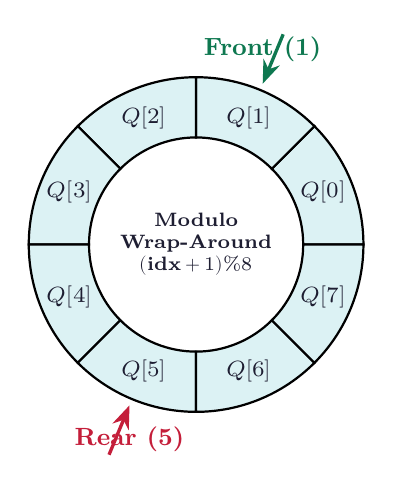
\begin{tikzpicture}[scale=0.85]
  % Draw circular ring segments
  \foreach \i in {0,1,...,7} {
    \draw[thick, fill=hdrteal] (\i*45:1.6cm) arc (\i*45:(\i+1)*45:1.6cm) -- 
          ({(\i+1)*45}:2.5cm) arc ({(\i+1)*45}:\i*45:2.5cm) -- cycle;
    \node[font=\footnotesize\bfseries, color=mydark] at (\i*45+22.5:2.05cm) {$Q[\i]$};
  }
  % Highlight front and rear
  \draw[-Stealth, very thick, color=mygreen] (67.5:3.4cm) -- (67.5:2.6cm) node[above=4pt, font=\small\bfseries] {Front (1)};
  \draw[-Stealth, very thick, color=myred] (247.5:3.4cm) -- (247.5:2.6cm) node[below=4pt, font=\small\bfseries] {Rear (5)};
  \node[font=\scriptsize\bfseries, color=mydark, align=center] at (0,0) {Modulo\\Wrap-Around\\$(\text{idx}+1)\%8$};
\end{tikzpicture}
\end{tcolorbox}

\subsection{Priority Queue}
A \textbf{Priority Queue} is an ADT where each element has an associated priority key. Elements are processed according to priority rather than arrival time:
\begin{itemize}[leftmargin=*, itemsep=3pt]
  \item \textbf{Ascending Priority Queue:} Item with the lowest numerical priority value is extracted first.
  \item \textbf{Descending Priority Queue:} Item with the highest numerical priority value is extracted first.
\end{itemize}

\par\vspace{6pt}\noindent
\begingroup
\setlength{\tabcolsep}{4.5pt}
\setlength{\extrarowheight}{3pt}
\renewcommand{\arraystretch}{1.3}
\begin{tabularx}{\linewidth}{|B{3.2cm}|B{3.0cm}|B{3.0cm}|Y|}
\hline
\textbf{Implementation} & \textbf{Enqueue Time} & \textbf{Dequeue Time} & \textbf{Trade-off Remarks} \\
\hline
Unordered Array & $\mathcal{O}(1)$ & $\mathcal{O}(n)$ & Linear search required to find extreme priority. \\
\hline
Ordered Array & $\mathcal{O}(n)$ & $\mathcal{O}(1)$ & Sorted insertion requires element shifts. \\
\hline
Unordered Linked List & $\mathcal{O}(1)$ & $\mathcal{O}(n)$ & Deletion requires traversing entire list. \\
\hline
Ordered Linked List & $\mathcal{O}(n)$ & $\mathcal{O}(1)$ & Dequeue is $\mathcal{O}(1)$ removal at head. \\
\hline
\textbf{Binary Heap} & $\mathbf{\mathcal{O}(\log n)}$ & $\mathbf{\mathcal{O}(\log n)}$ & \textbf{Optimal engineering balance} (standard in C++/Java). \\
\hline
\end{tabularx}
\endgroup

\subsection{Double-Ended Queue (DEQUE)}
A \textbf{DEQUE} (Double-Ended Queue) permits insertion and deletion at both the front and rear ends:
\begin{enumerate}[leftmargin=*, itemsep=3pt]
  \item \textbf{Input-Restricted DEQUE:} Insertion is allowed at only one end (e.g., rear), while deletion is allowed at both ends (front and rear).
  \item \textbf{Output-Restricted DEQUE:} Deletion is allowed at only one end (e.g., front), while insertion is allowed at both ends (front and rear).
\end{enumerate}

\newpage
% ===============================================================================
% MANDATORY QUICK REVISION PAGE
% ===============================================================================
\begin{center}
  {\large\bfseries\color{myred} Quick Revision --- Module 2}\\[3pt]
  {\small\color{mydark} Stacks and Queues: ADTs, Operations and Applications $|$ ES-CS301}
\end{center}
\noindent{\color{myred}\rule{\linewidth}{1.2pt}}
\vspace{4pt}

\begin{tcolorbox}[formulabox, title={\textbf{Key Formulas and Boundary Conditions at a Glance}}]
\renewcommand{\arraystretch}{1.25}
\begin{tabularx}{\linewidth}{B{5.0cm} X}
Stack Overflow / Underflow & $\text{Overflow: } \text{top} == \text{MAX} - 1, \quad \text{Underflow: } \text{top} == -1$ \\[2pt]
Linear Queue Full / Empty & $\text{Full: } \text{rear} == \text{MAX} - 1, \quad \text{Empty: } \text{front} == -1 \text{ or } \text{front} > \text{rear}$ \\[2pt]
Circular Queue Next Pointer & $\text{next} = (\text{index} + 1) \bmod \text{MAX}$ \\[2pt]
Circular Queue Full Condition & $(\text{rear} + 1) \bmod \text{MAX} == \text{front}$ \\[2pt]
Circular Queue Empty Condition & $\text{front} == -1$ \\[2pt]
Circular Queue Element Count & $\text{Count} = (\text{rear} - \text{front} + \text{MAX}) \bmod \text{MAX} + 1 \quad (\text{if non-empty})$ \\[2pt]
Stack Operation Complexities & $\text{Push: } \mathcal{O}(1), \quad \text{Pop: } \mathcal{O}(1), \quad \text{Peek: } \mathcal{O}(1)$ \\[2pt]
Binary Heap Priority Queue & $\text{Insert: } \mathcal{O}(\log n), \quad \text{Extract-Min/Max: } \mathcal{O}(\log n)$ \\[2pt]
\end{tabularx}
\end{tcolorbox}

\begin{tcolorbox}[defbox, title={\textbf{One-Line Definitions}}]
\begin{itemize}[leftmargin=*, itemsep=2pt, topsep=0pt]
  \item \textbf{Stack:} A linear data structure operating under the Last-In, First-Out (LIFO) discipline at a single end.
  \item \textbf{Queue:} A linear data structure operating under the First-In, First-Out (FIFO) discipline (front/rear).
  \item \textbf{False Overflow:} Rejection of enqueue requests in a linear queue when $\text{rear} == \text{MAX}-1$ despite empty slots at front.
  \item \textbf{Circular Queue:} A fixed-size queue that wraps around using modulo arithmetic to prevent memory drift.
  \item \textbf{Priority Queue:} An ADT where elements are retrieved based on an assigned priority key rather than FIFO arrival.
  \item \textbf{DEQUE:} A double-ended queue permitting insertion and deletion operations at both extremities.
  \item \textbf{Postfix Notation (RPN):} Parenthesis-free operator-after-operands notation evaluated in a single linear pass via a stack.
  \item \textbf{Activation Record:} A stack frame containing subroutine parameters, local variables, and return address.
\end{itemize}
\end{tcolorbox}

\newpage

\begin{tcolorbox}[exambox, title={\textbf{Frequently Asked / Viva Questions (Part 1)}}]
\begin{enumerate}[topsep=0pt, label=\textbf{Q\arabic*.}, itemsep=4pt]
  \item \Q{What is the primary difference between LIFO and FIFO operating principles?}
  LIFO (Last-In, First-Out), implemented by Stacks, ensures that the most recently inserted item is the first to be retrieved. FIFO (First-In, First-Out), implemented by Queues, guarantees that elements are serviced strictly in chronological order of arrival.

  \item \Q{Why are Postfix expressions preferred over Infix expressions by compiler evaluators?}
  Infix expressions require operator precedence tables, associativity rules, and parenthetical parsing, necessitating lookaheads and recursive evaluation. Postfix expressions are completely parenthesis-free and can be evaluated in a single linear pass ($\mathcal{O}(n)$ time) using an operand stack.

  \item \Q{How does a Circular Queue solve the False Overflow issue of a Linear Queue?}
  In a linear queue, deleted slots before \texttt{front} cannot be reused once \texttt{rear} reaches $\text{MAX}-1$. A circular queue treats the array as a closed ring using modulo arithmetic ($(\text{rear}+1) \bmod \text{MAX}$), wrapping new insertions into vacant slots at the beginning of the buffer.

  \item \Q{During postfix evaluation, why must the first popped element be assigned as the second operand?}
  Because stack operations are LIFO. If $A - B$ is converted to $A B -$, $B$ is pushed after $A$ and is therefore on top. Popping retrieves $B$ first ($\text{op}_2$) and $A$ second ($\text{op}_1$). For non-commutative operators (subtraction, division), swapping operands yields incorrect results ($\text{op}_1 - \text{op}_2 \ne \text{op}_2 - \text{op}_1$).

  \item \Q{State the condition for a Circular Queue of size $\text{MAX}$ to be completely full.}
  The standard condition is $(\text{rear} + 1) \bmod \text{MAX} == \text{front}$. This ensures that advancing the rear pointer by one slot would collide with the current front position.

  \item \Q{What is the difference between an Input-Restricted and an Output-Restricted DEQUE?}
  In an Input-Restricted DEQUE, insertions are permitted at only one end (e.g., rear), while deletions can occur at both ends (front and rear). In an Output-Restricted DEQUE, deletions are restricted to one end (e.g., front), while insertions can take place at both ends.

  \item \Q{How can a stack be used to check for balanced parentheses in an expression?}
  Traverse the expression character by character. When an opening delimiter (\texttt{(}, \texttt{[}, \texttt{\{}) is found, push it onto the stack. When a closing delimiter (\texttt{)}, \texttt{]}, \texttt{\}}) is found, pop the stack and check if it matches the closing symbol. If underflow occurs or types mismatch, it is unbalanced. The expression is balanced if the stack is empty at the end.
\end{enumerate}
\end{tcolorbox}

\newpage

\begin{tcolorbox}[exambox, title={\textbf{Frequently Asked / Viva Questions (Part 2)}}]
\begin{enumerate}[topsep=0pt, label=\textbf{Q\arabic*.}, itemsep=4pt, start=8]
  \item \Q{Why is a Binary Heap the preferred data structure for implementing a Priority Queue?}
  In an array or linked list, either insertion or extraction is $\mathcal{O}(n)$. A Binary Heap achieves an optimal compromise of $\mathcal{O}(\log n)$ for both insertion and extraction of the extreme-priority item, making it ideal for dynamic workloads.

  \item \Q{What happens to the call stack during infinite recursion, and what error is generated?}
  Each recursive call allocates an activation frame on the runtime call stack. Without a valid terminating base condition, stack frames accumulate until memory allocated for the call stack is exhausted, triggering a fatal \textbf{Stack Overflow} error.

  \item \Q{Can two stacks be implemented efficiently within a single one-dimensional array?}
  Yes. Stack 1 starts at index $0$ and grows rightward ($\text{top}_1++$), while Stack 2 starts at index $\text{MAX}-1$ and grows leftward ($\text{top}_2--$). Overflow occurs only when $\text{top}_1 + 1 == \text{top}_2$, maximizing total array space utilization.
\end{enumerate}
\end{tcolorbox}

\vspace{3pt}

\begin{tcolorbox}[tikzbox, title={\textbf{Summary Matrix: Comprehensive Comparison of Stack and Queue Structures}}]
\par\vspace{2pt}\noindent
\begingroup
\footnotesize
\setlength{\tabcolsep}{3.5pt}
\setlength{\extrarowheight}{1.5pt}
\renewcommand{\arraystretch}{1.15}
\begin{tabularx}{\linewidth}{|B{2.2cm}|B{3.2cm}|B{3.2cm}|Y|}
\hline
\textbf{Structure} & \textbf{Discipline / Pointers} & \textbf{Critical Conditions} & \textbf{Primary Practical Applications} \\
\hline
Stack & LIFO / FILO;\newline Single pointer $\text{top}$ & Full: $\text{top} == \text{MAX}-1$\newline Empty: $\text{top} == -1$ & Expression parsing, recursion, backtracking, undo operations. \\
\hline
Linear Queue & FIFO / LILO;\newline Two pointers $\text{front}, \text{rear}$ & Full: $\text{rear} == \text{MAX}-1$\newline Empty: $\text{front} == -1$ & Print spooling, simple task buffering (suffers memory drift). \\
\hline
Circular Queue & Ring FIFO;\newline Modulo wrap-around & Full: $(\text{rear}+1)\%\text{MAX} == \text{front}$\newline Empty: $\text{front} == -1$ & CPU scheduling (round robin), IO buffering, audio streaming. \\
\hline
Priority Queue & Priority-ordered;\newline Key-based selection & Governed by underlying heap/array capacity & Dijkstra's algorithm, Huffman coding, OS interrupt processing. \\
\hline
DEQUE & Double-ended;\newline Front \& Rear access & Full: depends on circular or linear array implementation & Browser tab history, job-stealing algorithms, palindrome verification. \\
\hline
\end{tabularx}
\endgroup
\end{tcolorbox}


% -- Module 3 -----------------------------------------------------------------
\modulestart{3}{Linked Lists Fundamentals and Singly Linked List (SLL)}

\section{Linked Lists Fundamentals and Singly Linked List (SLL)}
% ───────────────────────────────────────────────────────────────────────────────

\begin{tcolorbox}[defbox, title={\textbf{Definition: Singly Linked List (SLL) Architecture}}]
A \textbf{Singly Linked List} is a dynamic linear data structure composed of distinct nodes allocated at arbitrary non-contiguous physical memory locations. Each node consists of two essential components:
\begin{enumerate}[leftmargin=*, nosep]
  \item \textbf{Data Field:} Stores the actual information payload of type $T$.
  \item \textbf{Link (Next Pointer):} Stores the explicit physical memory address of the logically succeeding node.
\end{enumerate}
The list is anchored by an external pointer \texttt{head} referencing the first node. The terminal node's link contains \texttt{NULL}.
\end{tcolorbox}

\subsection{Limitations of Arrays vs Advantages of Linked Lists}
\begin{itemize}[leftmargin=*, itemsep=3pt]
  \item \textbf{Memory Allocation:} Arrays require fixed, compile-time contiguous memory allocation. Linked lists allocate memory dynamically on the heap at runtime via \texttt{malloc()} / \texttt{free()}, growing and shrinking on demand.
  \item \textbf{Insertion and Deletion Overhead:} Inserting or deleting an element at index $0$ in an array of size $n$ requires shifting all $n$ subsequent elements ($\mathcal{O}(n)$ time). In a linked list, inserting or deleting at the head requires updating pointer references, which executes in strictly $\mathbf{\mathcal{O}(1)}$ time without moving physical payloads.
  \item \textbf{Memory Fragmentation:} Arrays can suffer allocation failure due to external memory fragmentation even when total free RAM exceeds the array size; linked lists utilize scattered memory chunks effectively.
\end{itemize}

\begin{tcolorbox}[tikzbox, title={\textbf{Memory Representation and Pointer Rewiring in a Singly Linked List}}]
\centering
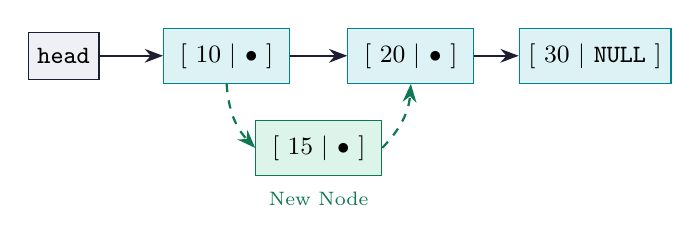
\begin{tikzpicture}[every node/.style={font=\small}, scale=0.9]
  % Head pointer
  \node[draw=mydark, fill=hdrgray, minimum size=0.6cm] (head) at (-1.5,0) {\texttt{head}};
  \node[llnode] (n1) at (0.8,0) {[ 10 $|$ $\bullet$ ]};
  \node[llnode] (n2) at (3.4,0) {[ 20 $|$ $\bullet$ ]};
  \node[llnode] (n3) at (6.0,0) {[ 30 $|$ \texttt{NULL} ]};

  \draw[arrow] (head) -- (n1.west);
  \draw[arrow] (n1.east) -- (n2.west);
  \draw[arrow] (n2.east) -- (n3.west);

  % Insertion example
  \node[llnode, draw=mygreen, fill=hdrgreen] (new) at (2.1,-1.3) {[ 15 $|$ $\bullet$ ]};
  \node[below=2pt, font=\scriptsize, color=mygreen] at (2.1,-1.7) {New Node};
  \draw[-Stealth, thick, color=mygreen, dashed] (n1.south) to[bend right=20] (new.west);
  \draw[-Stealth, thick, color=mygreen, dashed] (new.east) to[bend right=20] (n2.south);
\end{tikzpicture}
\end{tcolorbox}

\subsection{Singly Linked List Algorithmic Operations}
\begin{tcolorbox}[formulabox, title={\textbf{Algorithms for Insertion and Deletion in SLL}}]
\textbf{1. Insertion at Beginning ($\mathcal{O}(1)$):}
\begin{verbatim}
newNode = allocateNode(val);
newNode->next = head;
head = newNode;
\end{verbatim}

\textbf{2. Insertion at End ($\mathcal{O}(n)$ without tail pointer, $\mathcal{O}(1)$ with tail):}
\begin{verbatim}
newNode = allocateNode(val); newNode->next = NULL;
if (head == NULL) { head = newNode; return; }
ptr = head;
while (ptr->next != NULL) ptr = ptr->next;
ptr->next = newNode;
\end{verbatim}

\textbf{3. Deletion at Beginning ($\mathcal{O}(1)$):}
\begin{verbatim}
if (head == NULL) report "Underflow";
temp = head;
head = head->next;
free(temp);
\end{verbatim}

\textbf{4. Deletion of a Node with Value $X$ ($\mathcal{O}(n)$):}
\begin{verbatim}
if (head == NULL) return;
if (head->data == X) { temp = head; head = head->next; free(temp); return; }
curr = head; prev = NULL;
while (curr != NULL && curr->data != X) { prev = curr; curr = curr->next; }
if (curr == NULL) report "Key Not Found";
else { prev->next = curr->next; free(curr); }
\end{verbatim}
\end{tcolorbox}

% ───────────────────────────────────────────────────────────────────────────────
\section{Linked Representation of Stack and Queue \& Header Nodes}
% ───────────────────────────────────────────────────────────────────────────────

\subsection{Linked Stack and Linked Queue}
\begin{itemize}[leftmargin=*, itemsep=3pt]
  \item \textbf{Linked Stack:} Implemented by inserting and deleting strictly at the head node of the linked list:
  \begin{itemize}[leftmargin=*, nosep]
    \item $\text{Push}(x) \equiv \text{Insert at Beginning} \implies \mathbf{\mathcal{O}(1)}$
    \item $\text{Pop}() \equiv \text{Delete from Beginning} \implies \mathbf{\mathcal{O}(1)}$
    \item Overflow never occurs unless the system runs out of heap memory.
  \end{itemize}
  \item \textbf{Linked Queue:} Maintained via two external pointers: \texttt{front} and \texttt{rear}:
  \begin{itemize}[leftmargin=*, nosep]
    \item $\text{Enqueue}(x) \equiv \text{Insert at End (via \texttt{rear}->\texttt{next} = newNode; \texttt{rear} = newNode)} \implies \mathbf{\mathcal{O}(1)}$
    \item $\text{Dequeue}() \equiv \text{Delete at Head (via \texttt{front} = \texttt{front}->\texttt{next})} \implies \mathbf{\mathcal{O}(1)}$
  \end{itemize}
\end{itemize}

\subsection{Header Nodes in Linked Lists}
A \textbf{Header Node} is a dummy node placed at the very beginning of the linked list before the first actual data node:
\begin{itemize}[leftmargin=*, itemsep=2pt]
  \item \textbf{Grounded Header List:} Header node's link points to the first data node; the last node's link contains \texttt{NULL}.
  \item \textbf{Circular Header List:} The last node's link points back to the header node itself.
  \item \textbf{Key Advantages:}
  \begin{enumerate}[leftmargin=*, nosep]
    \item Eliminates special-case coding for operations at the head (head pointer never needs re-assignment).
    \item The list is never truly empty (\texttt{head != NULL} always holds; an empty list has \texttt{head->next == NULL} or \texttt{head->next == head}).
    \item The header node's data field can store metadata (e.g., total node count, maximum element).
  \end{enumerate}
\end{itemize}

% ───────────────────────────────────────────────────────────────────────────────
\section{Doubly Linked Lists (DLL) and Circular Linked Lists (CLL)}
% ───────────────────────────────────────────────────────────────────────────────

\subsection{Doubly Linked List (DLL)}
In a \textbf{Doubly Linked List}, each node contains three fields: \texttt{prev} pointer, \texttt{data}, and \texttt{next} pointer.
\par\vspace{4pt}
\begin{itemize}[leftmargin=*, itemsep=3pt]
  \item \textbf{Invariant:} $\texttt{p->next->prev} == \texttt{p}$ and $\texttt{p->prev->next} == \texttt{p}$.
  \item \textbf{Bidirectional Traversal:} Allows forward and reverse scanning from any arbitrary node.
  \item \textbf{$\mathcal{O}(1)$ Deletion Given Node Pointer:} Deleting node $P$ does not require searching for its predecessor:
  \begin{verbatim}
  P->prev->next = P->next;
  if (P->next != NULL) P->next->prev = P->prev;
  free(P);
  \end{verbatim}
  \item \textbf{Trade-off:} Extra memory overhead for backward pointers ($2\times$ pointer overhead per node) and additional pointer adjustments during insertions.
\end{itemize}

\subsection{Circular Linked Lists (CLL)}
In a \textbf{Circular Singly Linked List}, the last node's link points back to the first node.
\par\vspace{3pt}
\begin{itemize}[leftmargin=*, itemsep=3pt]
  \item \textbf{Tail Pointer Paradigm:} By maintaining a single pointer \texttt{tail} to the last node:
  \begin{itemize}[leftmargin=*, nosep]
    \item Last node is accessible in $\mathcal{O}(1)$ (\texttt{tail}).
    \item First node is accessible in $\mathcal{O}(1)$ (\texttt{tail->next}).
    \item Both insertion at head and insertion at tail execute in strictly $\mathbf{\mathcal{O}(1)}$ time!
  \end{itemize}
  \item \textbf{Applications:} Continuous cycling processes, round-robin CPU scheduling, multiplayer turn games.
\end{itemize}

\subsection{Polynomial Representation and Addition using Linked Lists}
A single-variable polynomial $P(x) = a_n x^{e_n} + a_{n-1} x^{e_{n-1}} + \dots + a_0 x^{e_0}$ is represented as a linked list where each node contains: \texttt{coeff} (coefficient), \texttt{exp} (exponent), and \texttt{next} pointer, maintained in strictly decreasing order of exponents.

\begin{tcolorbox}[defbox, title={\textbf{Algorithm: Polynomial Addition using Singly Linked Lists}}]
\textbf{Algorithm AddPolynomials($P_1, P_2$):}
\begin{enumerate}[leftmargin=*, nosep]
  \item Initialize pointers $p = P_1, \; q = P_2$, and an empty resultant list $P_3$.
  \item While $p \ne \text{NULL}$ and $q \ne \text{NULL}$:
  \begin{itemize}[leftmargin=*, nosep]
    \item \textbf{Case 1 ($p\to\text{exp} == q\to\text{exp}$):} Compute $\text{sum} = p\to\text{coeff} + q\to\text{coeff}$. If $\text{sum} \ne 0$, insert term $(\text{sum}, p\to\text{exp})$ into $P_3$. Advance $p = p\to\text{next}, \; q = q\to\text{next}$.
    \item \textbf{Case 2 ($p\to\text{exp} > q\to\text{exp}$):} Insert term $(p\to\text{coeff}, p\to\text{exp})$ into $P_3$. Advance $p = p\to\text{next}$.
    \item \textbf{Case 3 ($p\to\text{exp} < q\to\text{exp}$):} Insert term $(q\to\text{coeff}, q\to\text{exp})$ into $P_3$. Advance $q = q\to\text{next}$.
  \end{itemize}
  \item Copy any remaining terms from $p$ or $q$ to the tail of $P_3$. Return $P_3$.
\end{enumerate}
Time Complexity: $\mathbf{\mathcal{O}(m + n)}$ where $m, n$ are the number of non-zero terms in $P_1, P_2$.
\end{tcolorbox}

% ───────────────────────────────────────────────────────────────────────────────
\section{Tree Terminologies and Binary Tree Foundations}
% ───────────────────────────────────────────────────────────────────────────────

\begin{tcolorbox}[defbox, title={\textbf{Definition: Tree Data Structure and Core Terminologies}}]
A \textbf{Tree} is a non-linear, hierarchical data structure consisting of a collection of nodes connected by directed or undirected edges, such that there exists a unique root node $R$ and no cycles.
\par\vspace{4pt}
\begin{itemize}[leftmargin=*, itemsep=2pt]
  \item \textbf{Root:} The topmost ancestor node with in-degree 0 (no incoming parent edge).
  \item \textbf{Leaf (Terminal Node):} A node with out-degree 0 (no child nodes).
  \item \textbf{Degree of a Node:} The total number of subtrees or immediate children attached to that node.
  \item \textbf{Degree of a Tree:} The maximum degree among all nodes in the tree.
  \item \textbf{Level and Depth:} The root is at Level 0 (or 1). The depth of a node is the length of the path from the root to that node.
  \item \textbf{Height of a Tree ($h$):} The maximum depth among all nodes in the tree (length of the longest path from root to leaf).
\end{itemize}
\end{tcolorbox}

\subsection{Mathematical Properties of Binary Trees}
A \textbf{Binary Tree} is a finite tree in which every node has at most two children, distinguished as \textbf{left child} and \textbf{right child}.
\begin{tcolorbox}[formulabox, title={\textbf{Core Mathematical Theorems on Binary Trees}}]
\begin{enumerate}[leftmargin=*, itemsep=3pt]
  \item Maximum number of nodes at level $i$ (with root at level 0):
  \begin{equation}
    N_{\max}(i) = 2^i
  \end{equation}
  \item Maximum total nodes in a binary tree of height $h$:
  \begin{equation}
    N_{\max}(h) = \sum_{i=0}^h 2^i = 2^{h+1} - 1
  \end{equation}
  \item Minimum height of a binary tree with $n$ nodes:
  \begin{equation}
    h_{\min} = \lceil \log_2(n + 1) \rceil - 1
  \end{equation}
  \item \textbf{Leaf vs Degree-2 Nodes Theorem:} In any non-empty binary tree, the number of leaf nodes $n_0$ is exactly one more than the number of nodes with degree two ($n_2$):
  \begin{equation}
    \mathbf{n_0 = n_2 + 1}
  \end{equation}
  \textit{Proof:} Let total nodes be $n = n_0 + n_1 + n_2$. Total edges in a tree of $n$ nodes is $E = n - 1$. Also, each degree-1 node contributes 1 outgoing branch and each degree-2 node contributes 2 outgoing branches: $E = n_1 + 2n_2$. Equating the two expressions:
  \begin{equation*}
    n_0 + n_1 + n_2 - 1 = n_1 + 2n_2 \implies n_0 - 1 = n_2 \implies \mathbf{n_0 = n_2 + 1}
  \end{equation*}
\end{enumerate}
\end{tcolorbox}

\subsection{Binary Tree Classifications}
\begin{itemize}[leftmargin=*, itemsep=3pt]
  \item \textbf{Full (Strict / Proper) Binary Tree:} Every internal node has exactly two children ($0$ or $2$ children; no node has degree 1).
  \item \textbf{Complete Binary Tree:} All levels are completely filled except possibly the last level, where nodes are filled strictly from left to right without gaps. Foundation of array-based Binary Heaps.
  \item \textbf{Perfect Binary Tree:} All internal nodes have two children and all leaves reside at the same maximum depth (contains exactly $2^{h+1}-1$ nodes).
  \item \textbf{Degenerate (Skewed) Binary Tree:} Every internal node has only one child, degrading to a linear linked list ($\mathcal{O}(n)$ height).
\end{itemize}

\subsection{Binary Tree Traversals}
\begin{enumerate}[leftmargin=*, itemsep=3pt]
  \item \textbf{Preorder Traversal (D-L-R):} Process Data $\to$ Traverse Left subtree $\to$ Traverse Right subtree.
  \item \textbf{Inorder Traversal (L-D-R):} Traverse Left subtree $\to$ Process Data $\to$ Traverse Right subtree. Produces sorted sequence for a BST!
  \item \textbf{Postorder Traversal (L-R-D):} Traverse Left subtree $\to$ Traverse Right subtree $\to$ Process Data. Used for deleting tree bottom-up and expression evaluation.
  \item \textbf{Level-Order Traversal (BFS):} Visit nodes level by level from top to bottom, left to right, implemented using a FIFO Queue.
\end{enumerate}

% ───────────────────────────────────────────────────────────────────────────────
\section{Threaded Binary Tree}
% ───────────────────────────────────────────────────────────────────────────────

\begin{tcolorbox}[defbox, title={\textbf{Definition: Threaded Binary Tree}}]
In an $n$-node binary tree, exactly $2n$ pointer fields exist, of which $n-1$ point to children and $n+1$ are \texttt{NULL}. A \textbf{Threaded Binary Tree} utilizes these wasted null pointers:
\begin{itemize}[leftmargin=*, nosep]
  \item A \texttt{NULL} left pointer is converted into a \textbf{thread} pointing to the node's \textbf{Inorder Predecessor}.
  \item A \texttt{NULL} right pointer is converted into a \textbf{thread} pointing to the node's \textbf{Inorder Successor}.
\end{itemize}
Boolean tags (\texttt{lTag}, \texttt{rTag}) indicate whether the pointer field is a normal child link ($0$) or a thread ($1$).
\end{tcolorbox}

\textbf{Primary Advantage:} Enables complete Inorder traversal without requiring recursive calls or an auxiliary stack, utilizing $\mathbf{\mathcal{O}(1)}$ auxiliary memory space.

% ───────────────────────────────────────────────────────────────────────────────
\section{Binary Search Tree (BST)}
% ───────────────────────────────────────────────────────────────────────────────

\begin{tcolorbox}[defbox, title={\textbf{Definition: Binary Search Tree (BST) Invariant}}]
A \textbf{Binary Search Tree (BST)} is a binary tree in which every node $x$ satisfies the BST ordering property:
\begin{itemize}[leftmargin=*, nosep]
  \item For all nodes $y$ in the left subtree of $x$: $\text{Key}(y) < \text{Key}(x)$.
  \item For all nodes $z$ in the right subtree of $x$: $\text{Key}(z) > \text{Key}(x)$.
\end{itemize}
Duplicate keys are either disallowed or handled uniformly in right subtrees.
\end{tcolorbox}

\subsection{BST Operations and Recursive Algorithms}
\begin{tcolorbox}[formulabox, title={\textbf{Core Binary Search Tree Algorithms}}]
\textbf{1. Algorithm BST\_Search($root, K$):}
\begin{verbatim}
if (root == NULL || root->data == K) return root;
if (K < root->data) return BST_Search(root->left, K);
return BST_Search(root->right, K);
\end{verbatim}

\textbf{2. Algorithm BST\_Insert($root, K$):}
\begin{verbatim}
if (root == NULL) return createNode(K);
if (K < root->data) root->left = BST_Insert(root->left, K);
else if (K > root->data) root->right = BST_Insert(root->right, K);
return root;
\end{verbatim}

\textbf{3. Algorithm BST\_Delete($root, K$):}
\begin{verbatim}
if (root == NULL) return root;
if (K < root->data) root->left = BST_Delete(root->left, K);
else if (K > root->data) root->right = BST_Delete(root->right, K);
else {
    // Case 1: Leaf node or Case 2: One child
    if (root->left == NULL) {
        temp = root->right; free(root); return temp;
    } else if (root->right == NULL) {
        temp = root->left; free(root); return temp;
    }
    // Case 3: Two children
    temp = findMin(root->right); // Inorder Successor
    root->data = temp->data;
    root->right = BST_Delete(root->right, temp->data);
}
return root;
\end{verbatim}
Complexity: Average $\mathbf{\mathcal{O}(\log_2 n)}$, Worst (skewed tree) $\mathbf{\mathcal{O}(n)}$.
\end{tcolorbox}

% ───────────────────────────────────────────────────────────────────────────────
\section{AVL Tree (Self-Balancing Binary Search Tree)}
% ───────────────────────────────────────────────────────────────────────────────

\begin{tcolorbox}[defbox, title={\textbf{Definition: AVL Tree and Balance Factor}}]
An \textbf{AVL Tree} is a strictly height-balanced Binary Search Tree where the \textbf{Balance Factor ($BF$)} of every node $v$ is constrained to $\{-1, 0, +1\}$:
\begin{equation}
  BF(v) = h(\text{left subtree}) - h(\text{right subtree}) \in \{-1, 0, +1\}
\end{equation}
If an insertion or deletion causes $|BF(v)| \ge 2$, the tree is rebalanced locally via rotations.
\end{tcolorbox}

\subsection{AVL Rebalancing Rotations}
\begin{enumerate}[leftmargin=*, itemsep=4pt]
  \item \textbf{LL Rotation (Single Right Rotation):} Applied when insertion occurs in the left subtree of the left child ($BF = +2$, child $BF = +1$).
  \item \textbf{RR Rotation (Single Left Rotation):} Applied when insertion occurs in the right subtree of the right child ($BF = -2$, child $BF = -1$).
  \item \textbf{LR Rotation (Double Rotation):} Insertion in the right subtree of the left child ($BF = +2$, child $BF = -1$). First Left-rotate left child, then Right-rotate parent.
  \item \textbf{RL Rotation (Double Rotation):} Insertion in the left subtree of the right child ($BF = -2$, child $BF = +1$). First Right-rotate right child, then Left-rotate parent.
\end{enumerate}

\begin{tcolorbox}[examplebox, title={\textbf{Step-by-Step AVL Construction Walkthrough}}]
Construct an AVL tree by inserting keys: $10, 20, 30, 40, 50, 25$.
\begin{itemize}[leftmargin=*, nosep]
  \item Insert $10, 20$: Tree balanced.
  \item Insert $30$: Path $10 \to 20 \to 30$ causes $BF(10) = -2$ (RR violation). Perform \textbf{RR (Left Rotation)} on $10$: $20$ becomes root, with children $10$ (left) and $30$ (right).
  \item Insert $40$: Attached as right child of $30$. Balanced ($BF(20)=-1$).
  \item Insert $50$: Path $30 \to 40 \to 50$ causes $BF(30) = -2$ (RR violation). Perform \textbf{RR (Left Rotation)} on $30$: $40$ takes $30$'s position, children $30, 50$.
  \item Insert $25$: Attached as left child of $30$. Root $20$ now has $BF(20) = -2$, child $40$ has $BF(40) = +1$ (RL violation). Perform \textbf{RL Double Rotation}: Right-rotate $40$ then Left-rotate $20$. New root is $30$, left subtree rooted at $20$ (children $10, 25$), right subtree rooted at $40$ (child $50$). Tree is perfectly balanced!
\end{itemize}
\end{tcolorbox}

\begin{tcolorbox}[formulabox, title={\textbf{Height Bound and Complexity of AVL Trees}}]
The minimum number of nodes $N(h)$ in an AVL tree of height $h$ satisfies the Fibonacci recurrence:
\begin{equation}
  N(h) = N(h-1) + N(h-2) + 1, \quad N(0) = 1, \; N(1) = 2
\end{equation}
Solving this relation yields an asymptotic upper bound on height:
\begin{equation}
  h < 1.44 \log_2(n + 2) \implies \mathbf{h = \mathcal{O}(\log_2 n)}
\end{equation}
Consequently, Search, Insert, and Delete operations in an AVL tree are \textbf{guaranteed strictly $\mathbf{\mathcal{O}(\log n)}$} in both average and worst cases!
\end{tcolorbox}

% ───────────────────────────────────────────────────────────────────────────────
\section{Applications of Binary Trees: Expression Trees and Huffman Coding}
% ───────────────────────────────────────────────────────────────────────────────

\subsection{Expression Trees}
An \textbf{Expression Tree} is a binary tree representing an arithmetic or logical formula:
\begin{itemize}[leftmargin=*, nosep]
  \item \textbf{Leaves:} Distinct operands (variables or numerical constants).
  \item \textbf{Internal Nodes:} Binary operators ($+, -, *, /, \wedge$).
  \item \textbf{Traversals:} Inorder traversal with parentheses yields the equivalent \textbf{Infix} formula; Preorder traversal yields \textbf{Prefix}; Postorder traversal yields \textbf{Postfix}.
  \item \textbf{Construction Algorithm from Postfix:} Scan postfix expression token by token using a stack of tree node pointers. For an operand, create a leaf node and push pointer. For operator $\odot$, create an operator node, pop two nodes as right and left children, and push the newly formed subtree.
\end{itemize}

\subsection{Huffman Coding (Greedy Data Compression)}
\begin{tcolorbox}[defbox, title={\textbf{Huffman Algorithm for Optimal Prefix Codes}}]
Given an alphabet of $n$ symbols with given occurrence frequencies:
\begin{enumerate}[leftmargin=*, nosep]
  \item Create a Min-Priority Queue containing $n$ leaf nodes, each initialized with a symbol and its frequency.
  \item While the priority queue contains more than one node:
  \begin{itemize}[leftmargin=*, nosep]
    \item $left = \text{Extract-Min}()$
    \item $right = \text{Extract-Min}()$
    \item Allocate a new internal node $Z$ with $\text{freq}(Z) = \text{freq}(left) + \text{freq}(right)$.
    \item Set $Z\to\text{left} = left$ and $Z\to\text{right} = right$.
    \item $\text{Insert}(Z)$ back into the Min-Priority Queue.
  \end{itemize}
  \item The remaining single node is the root of the \textbf{Huffman Tree}.
  \item Assign binary bit \texttt{'0'} to each left branch and \texttt{'1'} to each right branch. Paths from root to leaves produce unambiguous \textbf{Prefix Codes} (no code is a prefix of another).
\end{enumerate}
Time Complexity: $\mathbf{\mathcal{O}(n \log_2 n)}$ using a binary min-heap.
\end{tcolorbox}

% ───────────────────────────────────────────────────────────────────────────────
\section{Multi-Way Search Trees: B-Tree and B+ Tree}
% ───────────────────────────────────────────────────────────────────────────────

\subsection{B-Tree of Order $m$}
Designed for secondary storage (disk systems) to minimize slow disk I/O operations by maximizing node branching factor.
\begin{tcolorbox}[defbox, title={\textbf{Axiomatic Properties of B-Tree of Order $m$}}]
\begin{enumerate}[leftmargin=*, nosep]
  \item Every node has at most $m$ children and $m - 1$ keys.
  \item The root node has at least $2$ children (unless it is a leaf).
  \item Every internal node (except root) has at least $\lceil m/2 \rceil$ children and $\lceil m/2 \rceil - 1$ keys.
  \item All leaf nodes reside at the exact same depth/level.
  \item A non-leaf node with $k$ children contains $k - 1$ keys acting as separation boundaries.
\end{enumerate}
\end{tcolorbox}

\begin{tcolorbox}[formulabox, title={\textbf{B-Tree Algorithmic Operations: Insertion and Deletion}}]
\textbf{1. B-Tree Insertion Algorithm:}
\begin{itemize}[leftmargin=*, nosep]
  \item Search to find the appropriate leaf node for key $K$.
  \item If leaf contains $< m - 1$ keys, insert $K$ into sorted position.
  \item \textbf{Node Splitting (Overflow):} If leaf already contains $m - 1$ keys, inserting $K$ causes overflow ($m$ keys). Split node around the \textbf{median key} at position $\lceil m/2 \rceil$:
  \begin{itemize}[leftmargin=*, nosep]
    \item Keys left of median form a new left leaf.
    \item Keys right of median form a new right leaf.
    \item Median key is \textbf{promoted} to the parent node.
    \item If parent overflows, propagate splitting upward recursively (if root splits, tree height increases by 1).
  \end{itemize}
\end{itemize}

\par\vspace{2pt}\noindent
\textbf{2. B-Tree Deletion Algorithm:}
\begin{itemize}[leftmargin=*, nosep]
  \item If key is in an internal node, replace it with its inorder predecessor or successor, reducing problem to deletion from a leaf.
  \item If leaf has $\ge \lceil m/2 \rceil$ keys, delete directly.
  \item \textbf{Underflow Handling ($< \lceil m/2 \rceil - 1$ keys):}
  \begin{itemize}[leftmargin=*, nosep]
    \item \textbf{Borrowing (Rotation):} If immediate sibling has $> \lceil m/2 \rceil - 1$ keys, borrow a key via rotation through parent.
    \item \textbf{Merging:} If both siblings have minimum keys, merge the node with a sibling and the intervening parent separator key (may cause underflow in parent).
  \end{itemize}
\end{itemize}
\end{tcolorbox}

\subsection{B+ Tree and Comparison with B-Tree}
\begin{itemize}[leftmargin=*, itemsep=3pt]
  \item \textbf{B+ Tree Structure:} In a B+ tree, all data records and actual keys are stored \textbf{strictly in leaf nodes}. Internal nodes store only search routing keys.
  \item \textbf{Linked Leaves:} All leaf nodes are linked sequentially via pointers to form a doubly linked list, enabling extremely fast $\mathcal{O}(k)$ range queries.
  \item \textbf{Database Indexing Standard:} B+ Trees are universally used in relational database engines (MySQL, PostgreSQL, Oracle) and file systems (NTFS, ext4).
\end{itemize}

\newpage
% ===============================================================================
% MANDATORY QUICK REVISION PAGE
% ===============================================================================
\begin{center}
  {\large\bfseries\color{myred} Quick Revision --- Module 3}\\[3pt]
  {\small\color{mydark} Linked Lists and Tree Data Structures $|$ ES-CS301}
\end{center}
\noindent{\color{myred}\rule{\linewidth}{1.2pt}}
\vspace{4pt}

\begin{tcolorbox}[formulabox, title={\textbf{Key Formulas, Tree Bounds and Complexity at a Glance}}]
\renewcommand{\arraystretch}{1.25}
\begin{tabularx}{\linewidth}{B{5.0cm} X}
Binary Tree Max Nodes Level $i$ / Total & $N_{\max}(i) = 2^i, \quad N_{\text{total}}(h) = 2^{h+1} - 1$ \\[2pt]
Leaf Nodes vs Degree-2 Nodes & $n_0 = n_2 + 1 \quad \text{(Universal Binary Tree Invariant)}$ \\[2pt]
Binary Tree Minimum Height & $h_{\min} = \lceil \log_2(n+1) \rceil - 1 \implies \Omega(\log n)$ \\[2pt]
AVL Balance Factor & $BF(v) = h_L(v) - h_R(v) \in \{-1, 0, +1\}$ \\[2pt]
AVL Maximum Height Bound & $h < 1.44 \log_2 n \implies \text{Guaranteed } \mathcal{O}(\log n)$ \\[2pt]
SLL Head Operations vs Search & $\text{Insert/Delete Head: } \mathcal{O}(1), \quad \text{Search/Tail: } \mathcal{O}(n)$ \\[2pt]
BST Search / Insert / Delete & Average: $\mathcal{O}(\log n), \quad \text{Worst (skewed): } \mathcal{O}(n)$ \\[2pt]
B-Tree Key Bounds per Node & $\lceil m/2 \rceil - 1 \le \text{keys} \le m - 1, \quad \text{Search: } \mathcal{O}(\log_m n)$ \\[2pt]
\end{tabularx}
\end{tcolorbox}

\begin{tcolorbox}[defbox, title={\textbf{One-Line Definitions}}]
\begin{itemize}[leftmargin=*, itemsep=2pt, topsep=0pt]
  \item \textbf{Singly Linked List:} A dynamic linear data structure composed of nodes storing data and a single pointer to the successor.
  \item \textbf{Doubly Linked List:} A linked list where each node contains pointers to both its forward and backward adjacent nodes.
  \item \textbf{Circular Linked List:} A linked list whose terminal node points back to the first node instead of storing \texttt{NULL}.
  \item \textbf{Header Node:} A dummy lead node placed before actual data elements to simplify edge cases and eliminate head pointer updates.
  \item \textbf{Complete Binary Tree:} A binary tree completely filled at all levels except possibly the last, which is filled left-to-right.
  \item \textbf{Threaded Binary Tree:} A binary tree that replaces null leaf pointers with threads to inorder predecessors and successors.
  \item \textbf{Binary Search Tree (BST):} A binary tree where all left descendants are smaller and all right descendants are greater than the node.
  \item \textbf{AVL Tree:} A height-balanced BST where the heights of left and right subtrees of every node differ by at most 1 ($|BF| \le 1$).
\end{itemize}
\end{tcolorbox}

\newpage

\begin{tcolorbox}[exambox, title={\textbf{Frequently Asked / Viva Questions (Part 1)}}]
\begin{enumerate}[topsep=0pt, label=\textbf{Q\arabic*.}, itemsep=4pt]
  \item \Q{State and prove the relationship between leaf nodes and degree-2 nodes in any non-empty binary tree.}
  In any binary tree, $n_0 = n_2 + 1$. Proof: Let total nodes be $n = n_0 + n_1 + n_2$. Total edges in a tree of $n$ nodes is $E = n - 1$. Also, each degree-1 node contributes 1 outgoing branch and each degree-2 node contributes 2: $E = n_1 + 2n_2$. Setting $n_0 + n_1 + n_2 - 1 = n_1 + 2n_2$ simplifies directly to $n_0 = n_2 + 1$.

  \item \Q{Why does Inorder traversal of a Binary Search Tree produce sorted output?}
  Inorder traversal follows the Left-Data-Right (L-D-R) sequence. Because the BST invariant guarantees that all left subtree nodes are smaller than the root, and the root is smaller than all right subtree nodes, recursively visiting Left, then Root, then Right naturally produces a monotonically ascending sequence.

  \item \Q{Explain the four rebalancing rotations of an AVL tree.}
  Single Right (LL) fixes left-heavy imbalance caused by insertion in left subtree of left child. Single Left (RR) fixes right-heavy imbalance. Left-Right (LR) double rotation fixes left-heavy node with right-heavy child via left rotation on child followed by right on parent. Right-Left (RL) performs right rotation on child followed by left on parent.

  \item \Q{How does a B+ Tree differ fundamentally from a B-Tree?}
  In a B-tree, keys and associated data records are stored in both internal and leaf nodes. In a B+ tree, all data records are stored strictly in leaf nodes; internal nodes store only routing index keys. Furthermore, leaf nodes in a B+ tree are linked sequentially into a linked list for rapid range scanning.

  \item \Q{What are the advantages of maintaining a Tail pointer in a Circular Linked List?}
  With only a tail pointer, the last node is directly accessed in $\mathcal{O}(1)$ via \texttt{tail}, and the first node is accessed in $\mathcal{O}(1)$ via \texttt{tail->next}. This allows insertion at the beginning and insertion at the end to both execute in strictly $\mathcal{O}(1)$ time without traversing the list.

  \item \Q{What is the primary motivation for using Threaded Binary Trees?}
  In a binary tree of $n$ nodes, $n+1$ pointer fields are wasted as \texttt{NULL}. Threaded trees replace these null pointers with threads pointing to inorder predecessors and successors, permitting full inorder traversal without recursion or an auxiliary stack ($\mathcal{O}(1)$ extra space).

  \item \Q{What is the worst-case time complexity of searching in a BST, and when does it occur?}
  The worst-case search complexity is $\mathcal{O}(n)$. This occurs when keys are inserted in strictly sorted or reverse-sorted order, causing the BST to degenerate into a skewed linear chain where height $h = n - 1$.
\end{enumerate}
\end{tcolorbox}

\newpage

\begin{tcolorbox}[exambox, title={\textbf{Frequently Asked / Viva Questions (Part 2)}}]
\begin{enumerate}[topsep=0pt, label=\textbf{Q\arabic*.}, itemsep=4pt, start=8]
  \item \Q{Why are B-Trees preferred over Binary Search Trees for database indexes on disk?}
  Disk access is significantly slower than RAM access. A BST has high height ($\mathcal{O}(\log_2 n)$), requiring many sequential disk seeks. A B-Tree has a high branching factor $m$ (order $m \approx 100 \text{ to } 1000$), keeping height very low ($\mathcal{O}(\log_m n)$), so only 2 to 3 disk I/O reads are needed to retrieve any record.

  \item \Q{Explain the three cases of node deletion in a Binary Search Tree.}
  Case 1: Leaf node (simply remove and nullify parent's pointer). Case 2: Node has one child (bypass node by connecting parent directly to child). Case 3: Node has two children (replace value with inorder successor or predecessor, then delete that node which has at most one child).

  \item \Q{What is the purpose of a Header Node in a linked list?}
  A header node simplifies boundary conditions: it ensures the list is never empty (head pointer never changes) and eliminates special-case logic for inserting or deleting at the front of the list.
\end{enumerate}
\end{tcolorbox}

\vspace{3pt}

\begin{tcolorbox}[tikzbox, title={\textbf{Summary Matrix: Comprehensive Comparison of Tree Data Structures}}]
\par\vspace{2pt}\noindent
\begingroup
\footnotesize
\setlength{\tabcolsep}{3.5pt}
\setlength{\extrarowheight}{1.5pt}
\renewcommand{\arraystretch}{1.15}
\begin{tabularx}{\linewidth}{|B{2.2cm}|B{3.2cm}|B{3.2cm}|Y|}
\hline
\textbf{Tree Structure} & \textbf{Structural Invariant} & \textbf{Search Complexity} & \textbf{Primary Application Domain} \\
\hline
Binary Tree & At most 2 children per node & $\mathcal{O}(n)$ & Expression trees, hierarchical parsing, Huffman coding. \\
\hline
Threaded Binary Tree & Null pointers store inorder links & Traversal: $\mathcal{O}(1)$ space & Stackless tree traversal in memory-constrained systems. \\
\hline
Binary Search Tree (BST) & $\text{Left} < \text{Root} < \text{Right}$ & Avg: $\mathcal{O}(\log n)$, Worst: $\mathcal{O}(n)$ & Dynamic searching, symbol tables, dictionary ADT. \\
\hline
AVL Tree & Strict balance: $|BF| \le 1$ & Guaranteed $\mathcal{O}(\log n)$ & Search-intensive in-memory datasets and lookup tables. \\
\hline
B-Tree & Multi-way: $\lceil m/2 \rceil \le \text{children} \le m$ & $\mathcal{O}(\log_m n)$ & File systems, relational databases, storage indexing. \\
\hline
B+ Tree & Data in leaves; leaves linked & $\mathcal{O}(\log_m n)$ & Database query engines, fast sequential range retrieval. \\
\hline
\end{tabularx}
\endgroup
\end{tcolorbox}


% -- Module 4 -----------------------------------------------------------------
\modulestart{4}{Classification and Criteria of Sorting Algorithms}

\section{Classification and Criteria of Sorting Algorithms}
% ───────────────────────────────────────────────────────────────────────────────

\begin{tcolorbox}[defbox, title={\textbf{Definition: Sorting Problem and Taxonomic Criteria}}]
Given a sequence of $n$ records $R_1, R_2, \dots, R_n$ with keys $K_1, K_2, \dots, K_n$, \textbf{sorting} is the algorithmic permutation of these records into an ordered sequence $R_{\pi(1)}, R_{\pi(2)}, \dots, R_{\pi(n)}$ such that:
\begin{equation}
  K_{\pi(1)} \le K_{\pi(2)} \le \dots \le K_{\pi(n)}
\end{equation}
\textbf{Core Taxonomic Criteria:}
\begin{enumerate}[leftmargin=*, nosep]
  \item \textbf{Internal vs External Sorting:} Internal sorting holds the entire dataset concurrently in main RAM. External sorting processes massive datasets residing on secondary storage (hard drives, tapes) using phased multi-way merge passes.
  \item \textbf{Space Efficiency (In-Place vs Out-of-Place):} An in-place algorithm requires strictly $\mathcal{O}(1)$ auxiliary space beyond the input buffer (e.g., Insertion Sort, Heap Sort). Out-of-place algorithms require $\mathcal{O}(n)$ auxiliary storage (e.g., Merge Sort).
  \item \textbf{Stability:} A sorting algorithm is \textbf{stable} if records with identical keys preserve their relative initial input ordering:
  \begin{equation}
    K_i = K_j \text{ with } i < j \implies \pi(i) < \pi(j)
  \end{equation}
  \item \textbf{Adaptivity:} An algorithm is adaptive if its runtime decreases when the input array is already partially or completely sorted (e.g., Bubble Sort with swap flag, Insertion Sort).
\end{enumerate}
\end{tcolorbox}

\begin{tcolorbox}[formulabox, title={\textbf{Theoretical Lower Bound for Comparison-Based Sorting}}]
Any deterministic comparison-based sorting algorithm can be modeled as a binary decision tree where each internal node represents a comparison $A[i] \le A[j]$ and each leaf represents one of the $n!$ possible permutations of the input.
\par\vspace{3pt}
For a binary tree of height $h$ with at least $n!$ leaves:
\begin{equation}
  2^h \ge n! \implies h \ge \log_2(n!)
\end{equation}
Applying Stirling's approximation ($\ln(n!) \approx n \ln n - n$):
\begin{equation}
  h \ge \sum_{k=1}^n \log_2 k \ge \sum_{k=n/2}^n \log_2\left(\frac{n}{2}\right) = \frac{n}{2} \log_2\left(\frac{n}{2}\right) = \mathbf{\Omega(n \log_2 n)}
\end{equation}
Thus, no comparison-based sorting algorithm can achieve a worst-case time complexity faster than $\mathbf{\Omega(n \log n)}$.
\end{tcolorbox}

% ───────────────────────────────────────────────────────────────────────────────
\section{Elementary Sorting Algorithms}
% ───────────────────────────────────────────────────────────────────────────────

\subsection{Selection Sort}
\begin{itemize}[leftmargin=*, itemsep=3pt]
  \item \textbf{Working Principle:} In each pass $i \in [0, n-2]$, find the minimum element in unsorted subarray $A[i \dots n-1]$ and swap it with $A[i]$.
  \item \textbf{Comparisons:} Total comparisons are fixed for all input distributions:
  \begin{equation}
    C(n) = \sum_{i=0}^{n-2} (n - 1 - i) = (n - 1) + (n - 2) + \dots + 1 = \frac{n(n - 1)}{2} = \mathbf{\Theta(n^2)}
  \end{equation}
  \item \textbf{Swaps:} At most $n - 1$ swaps ($\mathcal{O}(n)$ writes) --- ideal when write operations are physically expensive (e.g., EEPROM/Flash memory).
  \item \textbf{Properties:} In-place ($\mathcal{O}(1)$ space), \textbf{Unstable} (e.g., sorting $[4_a, 4_b, 2]$ swaps $4_a$ with $2$, placing $4_a$ after $4_b$).
\end{itemize}

\subsection{Bubble Sort}
\begin{itemize}[leftmargin=*, itemsep=3pt]
  \item \textbf{Working Principle:} Iteratively scan the array, comparing adjacent pairs $(A[j], A[j+1])$ and swapping them if out of order, bubbling the largest item to the end in each pass.
  \item \textbf{Optimization:} Maintain a boolean flag \texttt{swapped}. If no swaps occur in a full pass, the array is already sorted and the algorithm terminates immediately.
  \item \textbf{Complexity:} Best-case: $\mathbf{\mathcal{O}(n)}$ (with flag on sorted input). Average and Worst-case: $\mathbf{\mathcal{O}(n^2)}$ comparisons and swaps.
  \item \textbf{Properties:} In-place ($\mathcal{O}(1)$ space), \textbf{Stable}, Adaptive.
\end{itemize}

\subsection{Insertion Sort}
\begin{itemize}[leftmargin=*, itemsep=3pt]
  \item \textbf{Working Principle:} Simulates how cards are sorted in hand: incrementally pick $A[i]$ and insert it into its correct relative position within the sorted subarray $A[0 \dots i-1]$ by shifting larger elements one position to the right.
  \item \textbf{Complexity Analysis:}
  \begin{itemize}[leftmargin=*, nosep]
    \item \textbf{Best-Case (Sorted Input):} Only 1 comparison per element, 0 shifts $\implies \mathbf{\mathcal{O}(n)}$ time.
    \item \textbf{Worst-Case (Reverse-Sorted Input):} Max shifts: $\sum_{i=1}^{n-1} i = \frac{n(n-1)}{2} \implies \mathbf{\mathcal{O}(n^2)}$ time.
    \item \textbf{Average-Case:} $\frac{n(n-1)}{4} \text{ shifts} \implies \mathbf{\mathcal{O}(n^2)}$ time.
  \end{itemize}
  \item \textbf{Properties:} In-place ($\mathcal{O}(1)$ space), \textbf{Stable}, Online (can sort incoming streaming data), highly optimal for small arrays ($n \le 16$).
\end{itemize}

% ───────────────────────────────────────────────────────────────────────────────
\section{Advanced Divide-and-Conquer \& Tree-Based Sorting}
% ───────────────────────────────────────────────────────────────────────────────

\subsection{Quick Sort (Partition-Exchange Sort)}
\begin{tcolorbox}[defbox, title={\textbf{Quick Sort Principle and Partitioning Strategy}}]
Quick Sort operates on the \textbf{Divide-and-Conquer} paradigm:
\begin{enumerate}[leftmargin=*, nosep]
  \item \textbf{Partition:} Select a pivot element $P$. Rearrange array such that all elements $\le P$ precede $P$, and all elements $\ge P$ succeed $P$. The pivot $P$ settles into its final sorted position $q$.
  \item \textbf{Recurse:} Recursively apply Quick Sort to subarrays $A[\text{low} \dots q-1]$ and $A[q+1 \dots \text{high}]$.
\end{enumerate}
\par\vspace{2pt}\noindent
\textbf{Lomuto Partition Algorithm ($A, \text{low}, \text{high}$):}
\begin{verbatim}
pivot = A[high]; i = low - 1;
for j = low to high - 1 do:
    if (A[j] <= pivot) then:
        i = i + 1; swap(A[i], A[j]);
swap(A[i + 1], A[high]);
return (i + 1);
\end{verbatim}
\end{tcolorbox}

\begin{tcolorbox}[formulabox, title={\textbf{Quick Sort Recurrence Relations and Asymptotic Analysis}}]
\textbf{1. Best-Case Analysis (Balanced Partition):}
Pivot consistently bisects the array into two equal halves of size $n/2$:
\begin{equation}
  T(n) = 2 T\left(\frac{n}{2}\right) + \Theta(n) \implies \mathbf{T(n) = \Theta(n \log_2 n)}
\end{equation}

\textbf{2. Worst-Case Analysis (Extremely Unbalanced Partition):}
Occurs when the array is already sorted or reverse-sorted and the first or last element is chosen as pivot, yielding subproblems of size $0$ and $n-1$:
\begin{equation}
  T(n) = T(n - 1) + T(0) + \Theta(n) = T(n - 1) + c n = c \sum_{i=1}^n i \implies \mathbf{T(n) = \Theta(n^2)}
\end{equation}

\textbf{3. Average-Case Analysis:} Assuming all permutations equally probable: $\mathbf{\mathcal{O}(n \log n)}$.
\par\vspace{3pt}\noindent
\textbf{Auxiliary Space:} $\mathcal{O}(\log n)$ stack frames for balanced recursion; degrades to $\mathcal{O}(n)$ in worst case. Quick Sort is \textbf{Unstable}.
\end{tcolorbox}

\subsection{Merge Sort}
\begin{tcolorbox}[formulabox, title={\textbf{Merge Sort Algorithm and Guaranteed Bounds}}]
Merge Sort recursively divides the array into two equal halves until single-element subarrays are reached, then merges them in sorted order using an auxiliary buffer:
\begin{equation}
  T(n) = 2 T\left(\frac{n}{2}\right) + \Theta(n) \quad \forall n > 1, \quad T(1) = 0
\end{equation}
By the Master Theorem (Case 2: $a = 2, b = 2, f(n) = \Theta(n) = \Theta(n^{\log_2 2})$):
\begin{equation}
  \mathbf{T(n) = \Theta(n \log_2 n) \quad \text{in Best, Average, and Worst Cases!}}
\end{equation}
\par\vspace{2pt}\noindent
\textbf{Two-Way Merge Algorithm ($A, \text{low}, \text{mid}, \text{high}$):}
\begin{verbatim}
i = low; j = mid + 1; k = low;
while (i <= mid && j <= high) {
    if (A[i] <= A[j]) { B[k] = A[i]; i++; }
    else { B[k] = A[j]; j++; }
    k++;
}
while (i <= mid) { B[k] = A[i]; i++; k++; }
while (j <= high) { B[k] = A[j]; j++; k++; }
for (p = low; p <= high; p++) A[p] = B[p];
\end{verbatim}
\par\vspace{2pt}\noindent
\textbf{Key Trade-offs:}
\begin{itemize}[leftmargin=*, nosep]
  \item \textbf{Guaranteed Performance:} Never degrades to $\mathcal{O}(n^2)$.
  \item \textbf{Space Overhead:} Requires $\mathbf{\mathcal{O}(n)}$ auxiliary memory array.
  \item \textbf{Stability:} \textbf{Stable} (ideal for complex multi-attribute sorting).
  \item \textbf{Linked Lists:} Does not require random access; sorts linked lists in $\mathcal{O}(n \log n)$ time with $\mathcal{O}(1)$ extra space.
\end{itemize}
\end{tcolorbox}

\subsection{Heap Sort}
A \textbf{Binary Heap} is a Complete Binary Tree mapped sequentially into an array $A[0 \dots n-1]$ satisfying the Max-Heap property: $A[\text{parent}] \ge A[\text{child}]$.
\begin{itemize}[leftmargin=*, nosep]
  \item Array Index Mapping: $\text{Parent}(i) = \lfloor (i - 1)/2 \rfloor, \; \text{Left}(i) = 2i + 1, \; \text{Right}(i) = 2i + 2$.
\end{itemize}

\begin{tcolorbox}[defbox, title={\textbf{Heap Sort Procedures and Linear Build-Heap Proof}}]
\textbf{1. Max-Heapify($A, i, n$) ($\mathcal{O}(\log n)$):}
\begin{verbatim}
largest = i; left = 2*i + 1; right = 2*i + 2;
if (left < n && A[left] > A[largest]) largest = left;
if (right < n && A[right] > A[largest]) largest = right;
if (largest != i) {
    swap(A[i], A[largest]);
    Max-Heapify(A, largest, n);
}
\end{verbatim}
\par\vspace{2pt}\noindent
\textbf{2. Build-Max-Heap ($O(n)$):} Calls \texttt{Max-Heapify} on all internal nodes from $\lfloor n/2 \rfloor - 1$ down to $0$:
\begin{equation}
  \sum_{h=0}^{\lfloor \log_2 n \rfloor} \left\lceil \frac{n}{2^{h+1}} \right\rceil \mathcal{O}(h) = \mathcal{O}\left( n \sum_{h=0}^\infty \frac{h}{2^h} \right) = \mathcal{O}(n \cdot 2) = \mathbf{\mathcal{O}(n)}
\end{equation}
\textbf{3. Heap Sort Algorithm ($\mathcal{O}(n \log n)$):}
\begin{enumerate}[leftmargin=*, nosep]
  \item Build a Max-Heap from input array: $\mathcal{O}(n)$.
  \item For $i = n - 1$ down to $1$:
  \begin{itemize}[leftmargin=*, nosep]
    \item Swap root $A[0]$ (current maximum) with $A[i]$.
    \item Reduce heap size by 1.
    \item Call \texttt{Max-Heapify}($A, 0, i$): $\mathcal{O}(\log n)$.
  \end{itemize}
\end{enumerate}
\par\vspace{2pt}\noindent
\textbf{Complexity:} Best, Average, Worst time strictly $\mathbf{\mathcal{O}(n \log n)}$. In-place ($\mathbf{\mathcal{O}(1)}$ space). \textbf{Unstable}.
\end{tcolorbox}

\subsection{Comprehensive Sorting Comparison Matrix}
\par\vspace{6pt}\noindent
\begingroup
\setlength{\tabcolsep}{3.5pt}
\setlength{\extrarowheight}{2.5pt}
\renewcommand{\arraystretch}{1.25}
\begin{tabularx}{\linewidth}{|B{2.2cm}|B{1.8cm}|B{1.8cm}|B{1.8cm}|B{1.3cm}|B{1.3cm}|Y|}
\hline
\textbf{Algorithm} & \textbf{Best} & \textbf{Average} & \textbf{Worst} & \textbf{Space} & \textbf{Stable?} & \textbf{Primary Use Case} \\
\hline
Selection Sort & $\mathcal{O}(n^2)$ & $\mathcal{O}(n^2)$ & $\mathcal{O}(n^2)$ & $\mathcal{O}(1)$ & No & Minimal write operations. \\
\hline
Bubble Sort & $\mathcal{O}(n)$ & $\mathcal{O}(n^2)$ & $\mathcal{O}(n^2)$ & $\mathcal{O}(1)$ & Yes & Educational; nearly sorted data. \\
\hline
Insertion Sort & $\mathcal{O}(n)$ & $\mathcal{O}(n^2)$ & $\mathcal{O}(n^2)$ & $\mathcal{O}(1)$ & Yes & Small lists ($n \le 16$); streaming. \\
\hline
Quick Sort & $\mathcal{O}(n \log n)$ & $\mathcal{O}(n \log n)$ & $\mathcal{O}(n^2)$ & $\mathcal{O}(\log n)$ & No & Fastest general in-memory sort. \\
\hline
Merge Sort & $\mathcal{O}(n \log n)$ & $\mathcal{O}(n \log n)$ & $\mathcal{O}(n \log n)$ & $\mathcal{O}(n)$ & Yes & Linked lists; external sorting. \\
\hline
Heap Sort & $\mathcal{O}(n \log n)$ & $\mathcal{O}(n \log n)$ & $\mathcal{O}(n \log n)$ & $\mathcal{O}(1)$ & No & Guaranteed $\mathcal{O}(n \log n)$ in-place. \\
\hline
\end{tabularx}
\endgroup

% ───────────────────────────────────────────────────────────────────────────────
\section{Hashing Techniques and Collision Resolution}
% ───────────────────────────────────────────────────────────────────────────────

\begin{tcolorbox}[defbox, title={\textbf{Definition: Hashing, Hash Table and Load Factor}}]
\textbf{Hashing} is a transformation technique that maps large variable keys $K$ from a universe $U$ into fixed integer slot indices in a \textbf{Hash Table} $T[0 \dots m-1]$ via a mathematical \textbf{Hash Function} $h(K)$:
\begin{equation}
  h : U \longrightarrow \{0, 1, \dots, m - 1\}
\end{equation}
The \textbf{Load Factor ($\alpha$)} is the ratio of stored keys $n$ to table capacity $m$:
\begin{equation}
  \alpha = \frac{n}{m}
\end{equation}
A \textbf{Collision} occurs when two distinct keys hash to the same slot: $h(K_1) = h(K_2)$ for $K_1 \ne K_2$.
\end{tcolorbox}

\subsection{Standard Hash Functions}
\begin{enumerate}[leftmargin=*, itemsep=3pt]
  \item \textbf{Division Method:} $h(K) = K \bmod m$. The table size $m$ should be a prime number not close to a power of 2 or 10 to minimize clustering.
  \item \textbf{Mid-Square Method:} Square the key $K^2$, and extract $r$ middle digits/bits as the index. Table size $m = 2^r$.
  \item \textbf{Folding Method:} Partition $K$ into parts matching index digit length, then sum parts:
  \begin{itemize}[leftmargin=*, nosep]
    \item \textbf{Fold-Shift:} Add components directly: $h(K) = (p_1 + p_2 + \dots) \bmod m$.
    \item \textbf{Fold-Boundary:} Reverse the digits of the outer parts before adding.
  \end{itemize}
  \item \textbf{Multiplication Method:} $h(K) = \lfloor m (K A \bmod 1) \rfloor$, where $0 < A < 1$ (Knuth recommends $A \approx \frac{\sqrt{5}-1}{2} \approx 0.618033$).
\end{enumerate}

\subsection{Collision Resolution Techniques}
\begin{enumerate}[leftmargin=*, itemsep=4pt]
  \item \textbf{Separate Chaining (Open Hashing):} Each table slot is a header pointer to a linked list of records hashing to that slot.
  \begin{itemize}[leftmargin=*, nosep]
    \item Can accommodate $\alpha > 1$ (table never gets "full").
    \item Average search time: $\mathcal{O}(1 + \alpha)$.
  \end{itemize}
  \item \textbf{Open Addressing (Closed Hashing):} All records reside directly in the table array ($m \ge n \implies \alpha \le 1$). If collision occurs, search alternate slots via a systematic probe sequence $h(K, i)$:
  \begin{itemize}[leftmargin=*, itemsep=2pt]
    \item \textbf{Linear Probing:} $h(K, i) = (h'(K) + i) \bmod m$. Suffers from \textbf{Primary Clustering} (adjacent occupied slots merge into long chains, degrading search to $\mathcal{O}(n)$).
    \item \textbf{Quadratic Probing:} $h(K, i) = (h'(K) + c_1 i + c_2 i^2) \bmod m$. Eliminates primary clustering but suffers from \textbf{Secondary Clustering} (keys hashing to same initial slot trace identical probe paths).
    \item \textbf{Double Hashing:} $h(K, i) = (h_1(K) + i \cdot h_2(K)) \bmod m$. Probe offset depends on the key itself ($h_2(K)$). Completely eliminates both primary and secondary clustering! Condition: $\gcd(h_2(K), m) = 1$.
  \end{itemize}
\end{enumerate}

\begin{tcolorbox}[examplebox, title={\textbf{Exam Numerical: Collision Resolution Walkthrough}}]
\textbf{Problem:} Insert keys $K = \{23, 43, 13, 27\}$ into a hash table of size $m = 7$ using $h'(K) = K \bmod 7$.
\par\vspace{2pt}\noindent
\textbf{1. Under Linear Probing ($h(K, i) = (h'(K) + i) \bmod 7$):}
\begin{itemize}[leftmargin=*, nosep]
  \item $K = 23$: $h'(23) = 23 \bmod 7 = 2$. Slot 2 is empty $\implies T[2] = 23$.
  \item $K = 43$: $h'(43) = 43 \bmod 7 = 1$. Slot 1 is empty $\implies T[1] = 43$.
  \item $K = 13$: $h'(13) = 13 \bmod 7 = 6$. Slot 6 is empty $\implies T[6] = 13$.
  \item $K = 27$: $h'(27) = 27 \bmod 7 = 6$. \textbf{Collision at 6!} Probe $i=1$: $(6 + 1) \bmod 7 = 0$. Slot 0 is empty $\implies T[0] = 27$.
\end{itemize}
\textbf{Final Table:} $T[0]=27, \; T[1]=43, \; T[2]=23, \; T[6]=13$.
\end{tcolorbox}

% ───────────────────────────────────────────────────────────────────────────────
\section{Graph Theory, Representations and Traversals}
% ───────────────────────────────────────────────────────────────────────────────

\begin{tcolorbox}[defbox, title={\textbf{Definition: Graph Data Structure and Core Terminologies}}]
A \textbf{Graph} $G = (V, E)$ consists of a non-empty finite set of vertices $V$ and a set of edges $E$ connecting pairs of vertices.
\begin{itemize}[leftmargin=*, itemsep=2pt]
  \item \textbf{Handshaking Lemma:} In any undirected graph:
  \begin{equation}
    \sum_{v \in V} \deg(v) = 2 |E|
  \end{equation}
  \textit{Corollary:} In any graph, the number of vertices with odd degree is always even.
  \item \textbf{Complete Graph $K_n$:} Every pair of distinct vertices is connected by a unique edge: $|E| = \frac{n(n-1)}{2}$.
  \item \textbf{Connected Component:} A maximal connected subgraph of an undirected graph.
  \item \textbf{Strongly Connected Digraph:} A directed graph where there exists a directed path between every ordered pair of vertices $(u, v)$.
\end{itemize}
\end{tcolorbox}

\subsection{Graph Storage Representations}
\par\vspace{4pt}\noindent
\begingroup
\setlength{\tabcolsep}{4.5pt}
\setlength{\extrarowheight}{3pt}
\renewcommand{\arraystretch}{1.3}
\begin{tabularx}{\linewidth}{|B{3.2cm}|B{2.8cm}|B{3.0cm}|Y|}
\hline
\textbf{Representation} & \textbf{Space Complexity} & \textbf{Edge Lookup $(u, v)$} & \textbf{Optimal Suitability} \\
\hline
\textbf{Adjacency Matrix} & $\mathcal{O}(V^2)$ & $\mathcal{O}(1)$ & Dense graphs ($|E| \approx |V|^2$); fast edge tests. \\
\hline
\textbf{Adjacency List} & $\mathcal{O}(V + E)$ & $\mathcal{O}(\deg(u))$ & Sparse graphs ($|E| \ll |V|^2$); DFS/BFS algorithms. \\
\hline
\textbf{Incidence Matrix} & $\mathcal{O}(V \cdot E)$ & $\mathcal{O}(E)$ & Theoretical network flows; hypergraphs. \\
\hline
\end{tabularx}
\endgroup

\subsection{Graph Search and Traversal Algorithms}
\begin{tcolorbox}[formulabox, title={\textbf{Breadth-First Search (BFS) and Depth-First Search (DFS) Algorithms}}]
\textbf{1. Algorithm BFS($G, s$):}
\begin{verbatim}
initialize boolean visited[V] = false, Queue Q;
visited[s] = true; Enqueue(Q, s);
while (!IsEmpty(Q)) {
    u = Dequeue(Q); print(u);
    for each vertex v adjacent to u:
        if (!visited[v]) {
            visited[v] = true; Enqueue(Q, v);
        }
}
\end{verbatim}
Time: $\mathbf{\mathcal{O}(V + E)}$ (Adjacency List), $\mathcal{O}(V^2)$ (Matrix) \quad Space: $\mathcal{O}(V)$
\par\vspace{3pt}\noindent
\textbf{2. Algorithm DFS($G, u$):}
\begin{verbatim}
visited[u] = true; print(u);
for each vertex v adjacent to u:
    if (!visited[v]) {
        DFS(G, v); // Recursive tree exploration
    }
\end{verbatim}
Time: $\mathbf{\mathcal{O}(V + E)}$ \quad Space: $\mathcal{O}(V)$ (System recursion stack)
\par\vspace{2pt}\noindent
\textbf{Edge Classification in DFS:} Tree edges (forming DFS forest), Back edges (to ancestor $\implies$ cycle detected!), Forward edges (to descendant), Cross edges (between distinct subtrees).
\end{tcolorbox}

\newpage
% ===============================================================================
% MANDATORY QUICK REVISION PAGE
% ===============================================================================
\begin{center}
  {\large\bfseries\color{myred} Quick Revision --- Module 4}\\[3pt]
  {\small\color{mydark} Sorting, Hashing and Graph Theory $|$ ES-CS301}
\end{center}
\noindent{\color{myred}\rule{\linewidth}{1.2pt}}
\vspace{4pt}

\begin{tcolorbox}[formulabox, title={\textbf{Key Formulas, Recurrences and Complexities at a Glance}}]
\renewcommand{\arraystretch}{1.25}
\begin{tabularx}{\linewidth}{B{5.0cm} X}
Comparison Sort Lower Bound & $\Omega(n \log_2 n) \quad \text{via Decision Tree Height } h \ge \log_2(n!)$ \\[2pt]
Merge Sort Recurrence & $T(n) = 2T(n/2) + \Theta(n) \implies \Theta(n \log_2 n) \quad \text{(Guaranteed)}$ \\[2pt]
Quick Sort Recurrences & $T_{\text{avg}}(n) = 2T(n/2) + \Theta(n) \implies \Theta(n \log_2 n), \quad T_{\text{worst}}(n) = \Theta(n^2)$ \\[2pt]
Linear Build-Heap Bound & $\sum_{h=0}^{\log n} \frac{n}{2^{h+1}} \mathcal{O}(h) = \mathcal{O}(n) \quad \text{(Linear Time Proof)}$ \\[2pt]
Hash Table Load Factor & $\alpha = n / m \quad (\alpha \le 1 \text{ for open addressing, } \alpha > 1 \text{ for chaining})$ \\[2pt]
Double Hashing Probe Offset & $h(K, i) = (h_1(K) + i \cdot h_2(K)) \bmod m \quad (h_2(K) \text{ coprime to } m)$ \\[2pt]
Graph Handshaking Lemma & $\sum_{v \in V} \deg(v) = 2 |E| \implies \text{Number of odd-degree vertices is even}$ \\[2pt]
BFS / DFS Traversal Time & $\mathcal{O}(V + E) \quad \text{(Adjacency List)}, \quad \mathcal{O}(V^2) \quad \text{(Adjacency Matrix)}$ \\[2pt]
\end{tabularx}
\end{tcolorbox}

\begin{tcolorbox}[defbox, title={\textbf{One-Line Definitions}}]
\begin{itemize}[leftmargin=*, itemsep=2pt, topsep=0pt]
  \item \textbf{Stable Sort:} A sorting algorithm that strictly preserves the relative input order of records with duplicate keys.
  \item \textbf{In-Place Sort:} A sorting algorithm requiring strictly $\mathcal{O}(1)$ auxiliary memory space beyond the input buffer.
  \item \textbf{Max-Heap:} A complete binary tree where key of every parent node is greater than or equal to its children ($A[\text{parent}(i)] \ge A[i]$).
  \item \textbf{Primary Clustering:} The undesirable tendency in linear probing where occupied adjacent slots coalesce into large continuous blocks.
  \item \textbf{Double Hashing:} An open addressing collision resolution technique where probe step size is calculated by an independent secondary hash function.
  \item \textbf{Adjacency List:} An array of linked lists where list $i$ stores all adjacent neighbors of vertex $i$, requiring optimal $\mathcal{O}(V + E)$ space.
  \item \textbf{Breadth-First Search (BFS):} Concentric layer-by-layer graph traversal implemented via a FIFO queue; yields shortest paths in unweighted graphs.
  \item \textbf{Depth-First Search (DFS):} Deep branch backtracking traversal using recursion/stack; detects cycles definitively via back edges.
\end{itemize}
\end{tcolorbox}

\newpage

\begin{tcolorbox}[exambox, title={\textbf{Frequently Asked / Viva Questions (Part 1)}}]
\begin{enumerate}[topsep=0pt, label=\textbf{Q\arabic*.}, itemsep=4pt]
  \item \Q{Why can comparison-based sorting algorithms not execute faster than $\mathcal{O}(n \log n)$ in the worst case?}
  Every comparison sort can be modeled as a decision tree with $n!$ leaves corresponding to all permutations. A binary tree of height $h$ has at most $2^h$ leaves. Therefore, $2^h \ge n! \implies h \ge \log_2(n!) \approx n \log_2 n - n \log_2 e = \Omega(n \log n)$. The height represents the worst-case number of comparisons.

  \item \Q{Under what conditions does Quick Sort degrade to its worst-case $\mathcal{O}(n^2)$ time?}
  When the partition is maximally unbalanced (e.g., one subproblem of size $n-1$ and one of size $0$). This occurs when the array is already sorted or reverse-sorted and the first or last element is consistently selected as the pivot.

  \item \Q{Why is Heap construction (\texttt{Build-Max-Heap}) $\mathcal{O}(n)$ rather than $\mathcal{O}(n \log n)$?}
  Although \texttt{Max-Heapify} takes $\mathcal{O}(h)$ time, most nodes in a binary tree reside near the leaves with very small heights $h$. Summing the cost across all heights $\sum_{h=0}^{\lfloor \log n \rfloor} \frac{n}{2^{h+1}} h = \frac{n}{2} \sum \frac{h}{2^h} = \frac{n}{2} \cdot 2 = \mathcal{O}(n)$.

  \item \Q{Compare Separate Chaining and Open Addressing for collision resolution.}
  Separate Chaining uses external linked lists for colliding elements; it never suffers from table overflow and handles load factor $\alpha > 1$. Open Addressing stores all elements directly within the array table ($\alpha \le 1$); it eliminates pointer memory overhead but requires collision probing and can suffer from clustering.

  \item \Q{What is the difference between Primary Clustering and Secondary Clustering?}
  Primary clustering occurs in linear probing when different keys hashing to adjacent slots merge into a single long contiguous chain. Secondary clustering occurs in quadratic probing when two distinct keys having the same initial hash index trace the exact same probe sequence.

  \item \Q{State the Handshaking Lemma and explain its primary corollary.}
  The Handshaking Lemma states that in any undirected graph, $\sum_{v \in V} \deg(v) = 2|E|$, because each edge contributes 1 degree to two incident vertices. The corollary is that the number of vertices with odd degree in any graph must be strictly even.

  \item \Q{Compare Adjacency Matrix and Adjacency List representations of a graph.}
  Adjacency Matrix uses $\mathcal{O}(V^2)$ space and checks edge existence in $\mathcal{O}(1)$ time; it is optimal for dense graphs ($|E| \approx |V|^2$). Adjacency List uses $\mathcal{O}(V + E)$ space and finds neighbors in $\mathcal{O}(\deg(v))$ time; it is optimal for sparse graphs ($|E| \ll |V|^2$).
\end{enumerate}
\end{tcolorbox}

\newpage

\begin{tcolorbox}[exambox, title={\textbf{Frequently Asked / Viva Questions (Part 2)}}]
\begin{enumerate}[topsep=0pt, label=\textbf{Q\arabic*.}, itemsep=4pt, start=8]
  \item \Q{How does DFS detect cycles in a directed graph?}
  During DFS traversal, vertices are colored White (unvisited), Gray (in active recursion stack), and Black (completely processed). If an edge $(u, v)$ encounters a Gray vertex $v$, that edge is a \textbf{Back Edge}, which definitively indicates the presence of a directed cycle.

  \item \Q{Why is Merge Sort preferred over Quick Sort for sorting linked lists?}
  In linked lists, random access is not available, which makes Quick Sort partitioning slow. Merge Sort divides a linked list in $\mathcal{O}(n)$ using the slow-fast pointer technique, and merges two sorted lists in $\mathcal{O}(n)$ time and strictly $\mathcal{O}(1)$ auxiliary space without requiring contiguous arrays.

  \item \Q{What is Topological Sorting, and what type of graph is required?}
  Topological sorting is a linear ordering of vertices such that for every directed edge $(u, v)$, vertex $u$ appears before $v$. It is strictly defined only on a \textbf{Directed Acyclic Graph (DAG)}.
\end{enumerate}
\end{tcolorbox}

\vspace{3pt}

\begin{tcolorbox}[tikzbox, title={\textbf{Summary Matrix: Comprehensive Comparison of Sorting, Hashing and Graphs}}]
\par\vspace{2pt}\noindent
\begingroup
\footnotesize
\setlength{\tabcolsep}{3.5pt}
\setlength{\extrarowheight}{1.5pt}
\renewcommand{\arraystretch}{1.15}
\begin{tabularx}{\linewidth}{|B{2.2cm}|B{3.2cm}|B{3.3cm}|Y|}
\hline
\textbf{Technique / Topic} & \textbf{Core Mechanism} & \textbf{Time / Space Complexity} & \textbf{Key Practical Application} \\
\hline
Quick Sort & Divide-and-Conquer;\newline Pivot partitioning & Avg: $\mathcal{O}(n \log n)$, Worst: $\mathcal{O}(n^2)$\newline Space: $\mathcal{O}(\log n)$ stack & Fastest general in-memory primitive data sorting. \\
\hline
Merge Sort & Divide-and-Conquer;\newline Two-finger merge & Best/Avg/Worst: $\mathcal{O}(n \log n)$\newline Space: $\mathcal{O}(n)$ auxiliary & External storage sorting, linked list sorting. \\
\hline
Heap Sort & Binary Max-Heap;\newline Root-leaf exchange & Guaranteed $\mathcal{O}(n \log n)$ all cases\newline Space: $\mathcal{O}(1)$ in-place & Systems where guaranteed $\mathcal{O}(n \log n)$ and minimal memory are required. \\
\hline
Double Hashing & Secondary hash step;\newline $h_1(K) + i \cdot h_2(K)$ & Search: $\mathcal{O}(1)$ avg, Worst: $\mathcal{O}(m)$\newline Space: $\mathcal{O}(m)$ array & Hash tables requiring zero primary/secondary clustering. \\
\hline
BFS & FIFO Queue;\newline Level-order expansion & $\mathcal{O}(V + E)$ (with Adj List)\newline Space: $\mathcal{O}(V)$ queue & Shortest paths in unweighted graphs, web crawlers. \\
\hline
DFS & LIFO Stack / Recursion;\newline Deep path exploration & $\mathcal{O}(V + E)$ (with Adj List)\newline Space: $\mathcal{O}(V)$ stack & Cycle detection, topological sorting, connected components. \\
\hline
\end{tabularx}
\endgroup
\end{tcolorbox}


\end{document}
